% =======================================================
% =======         HEADER FOR DOCUMENT        ============
% =======================================================
    
    % *********  SPECIFIC FOR THIS BOOK  ********
    \def\ProjectAuthorLink{https://github.com/SoyOscarRH}
    \def\ProjectNameLink{/}    
    

    % *********   DOCUMENT ITSELF   **************
    \documentclass[12pt, fleqn]{report}                             %Type of doc and size of font and left equations
    \usepackage[margin=1.2in]{geometry}                             %Margins and Geometry pacakge
    \usepackage{ifthen}                                             %Allow simple programming using if - then
    \usepackage[hidelinks]{hyperref}                                %Allow to create hiperlinks and Fuck Firefox
    \usepackage{pdfpages}                                           %Allow us 'import' PDF's
    \hypersetup{pageanchor=false}                                   %Solve 'double page 1' warnings in build :v
    \setlength{\parindent}{0pt}                                     %Eliminate ugly indentation
    \author{Oscar Andrés Rosas}                                     %Who I am

    \usepackage{subcaption}

    % *********   LANGUAJE    *****************
    \usepackage[spanish]{babel}                                     %Please allow me to type in spanish
    \usepackage[utf8]{inputenc}                                     %Lets use UFT-8
    \usepackage[T1]{fontenc}                                        %Allow for better font support
    \usepackage{textcmds}                                           %Allow us to use quoutes
    \usepackage{changepage}                                         %Allow us to use identate paragraphs
    \usepackage{anyfontsize}                                        %All the sizes for fonts wiiiii!

    % *********   MATH AND HIS STYLE  *********
    \usepackage{ntheorem, amsmath, amssymb, amsfonts}               %All fucking math, I want all!
    \usepackage{mathrsfs, mathtools, empheq}                        %All fucking math, I want all!
    \usepackage{cancel}                                             %Negate symbol
    \usepackage{centernot}                                          %Allow me to negate a symbol
    \decimalpoint                                                   %Use decimal point

    % *********   GRAPHICS AND IMAGES *********
    \usepackage{graphicx}                                           %Allow to create graphics
    \usepackage{float}                                              %For images
    \usepackage{wrapfig}                                            %Allow to create images
    \graphicspath{ {Graphics/} }                                    %Where are the images :D

    % *********   LISTS AND TABLES ***********
    \usepackage{listings, listingsutf8}                             %We will be using code here
    \usepackage[inline]{enumitem}                                   %We will need to enumarate
    \usepackage{tasks}                                              %Horizontal lists
    \usepackage{longtable}                                          %Lets make tables awesome
    \usepackage{booktabs}                                           %Lets make tables awesome
    \usepackage{tabularx}                                           %Lets make tables awesome
    \usepackage{multirow}                                           %Lets make tables awesome
    \usepackage{multicol}                                           %Create multicolumns

    % *********   REMOVE SOME ERRORS **********
    \hbadness=10000                                                 %Ignore \vbox and \hbox warings
    \hfuzz=\maxdimen\newdimen\hfuzz                                 %Ignore \vbox and \hbox warings

    % *********   HEADERS AND FOOTERS ********
    \usepackage{fancyhdr}                                           %Lets make awesome headers/footers
    \pagestyle{fancy}                                               %Lets make awesome headers/footers
    \setlength{\headheight}{16pt}                                   %Top line
    \setlength{\parskip}{0.5em}                                     %Top line
    \renewcommand{\footrulewidth}{0.5pt}                            %Bottom line

    \lhead {                                                        %Left Header
        \hyperlink{chapter.\arabic{chapter}}                        %Make a link to the current chapter
        {\normalsize{\textsc{\nouppercase{\leftmark}}}}             %And fot it put the name
    }

    \rhead {                                                        %Right Header
        \hyperlink{section.\arabic{chapter}.\arabic{section}}       %Make a link to the current chapter
            {\footnotesize{\textsc{\nouppercase{\rightmark}}}}      %And fot it put the name
    }

    \rfoot{\textsc{\small{\hyperref[sec:Index]{Ve al Índice}}}}     %This will always be a footer  

    \fancyfoot[L]{                                                  %Algoritm for a changing footer
        \ifthenelse{\isodd{\value{page}}}                           %IF ODD PAGE:
            {\href{https://SoyOscarRH.github.io/}                   %DO THIS:
                {\footnotesize                                      %Send the page
                    {\textsc{Oscar Andrés Rosas}}}}                 %Send the page
            {\href{https://compilandoconocimiento.com}              %ELSE DO THIS: 
                {\footnotesize                                      %Send the author
                    {\textsc{Machine Learning}}}}            %Send the author
    }
    
    
% =======================================================
% ===================   COMMANDS    =====================
% =======================================================

    % =========================================
    % =======   NEW ENVIRONMENTS   ============
    % =========================================
    \newenvironment{Indentation}[1][0.75em]                         %Use: \begin{Inde...}[Num]...\end{Inde...}
        {\begin{adjustwidth}{#1}{}}                                 %If you dont put nothing i will use 0.75 em
        {\end{adjustwidth}}                                         %This indentate a paragraph
    
    \newenvironment{SmallIndentation}[1][0.75em]                    %Use: The same that we upper one, just 
        {\begin{adjustwidth}{#1}{}\begin{footnotesize}}             %footnotesize size of letter by default
        {\end{footnotesize}\end{adjustwidth}}                       %that's it
    
    \def \Eq {equation}                                             %Stupid Visual studio error
    \newenvironment{MultiLineEquation}[1]                           %Use: To create MultiLine equations
        {\begin{\Eq}\begin{alignedat}{#1}}                          %Use: \begin{Multi..}{Num. de Columnas}
        {\end{alignedat}\end{\Eq}}                                  %And.. that's it!
    
    \newenvironment{MultiLineEquation*}[1]                          %Use: To create MultiLine equations
        {\begin{\Eq*}\begin{alignedat}{#1}}                         %Use: \begin{Multi..}{Num. de Columnas}
        {\end{alignedat}\end{\Eq*}}                                 %And.. that's it!

    \newenvironment{largeEq} {\begingroup \large}{\endgroup}        %Make eq bigger
    \newenvironment{LargeEq} {\begingroup \Large}{\endgroup}        %Make eq bigger
    \newenvironment{HugeEq} {\begingroup \Huge}{\endgroup}          %Make eq bigger!

    % =========================================
    % == GENERAL TEXT & SYMBOLS ENVIRONMENTS ==
    % =========================================
    
    % =====  TEXT  ======================
    \newcommand \Quote              {\qq}                           %Use: \Quote to use quotes
    \newcommand \Over               {\overline}                     %Use: \Bar to use just for short
    \newcommand \ForceNewLine       {$\Space$\\}                    %Use it in theorems for example
    \newcommand \ForceColumnBreak   {\vfill\null\columnbreak}       %Use only in multicols
    \newcommand \Link[2] {\underline{\texttt{\href{#1}{#2}}}}       %Use a link

    % =====  SPACES  ====================
    \DeclareMathOperator \Space     {\quad}                         %Use: \Space for a cool mega space
    \DeclareMathOperator \MegaSpace {\quad \quad}                   %Use: \MegaSpace for a cool mega mega space
    \DeclareMathOperator \MiniSpace {\;}                            %Use: \Space for a cool mini space
    
    % =====  MATH TEXT  =================
    \newcommand \Such           {\MiniSpace | \MiniSpace}           %Use: \Such like in sets
    \newcommand \Also           {\MiniSpace \text{y} \MiniSpace}    %Use: \Also so it's look cool
    \newcommand \Remember[1]    {\Space\text{\scriptsize{#1}}}      %Use: \Remember so it's look cool
    
    % =====  THEOREMS: IN SPANISH :0  ===
    \newtheorem{Theorem}        {Teorema}[section]                  %Use: \begin{Theorem}[Name]\label{Nombre}...
    \newtheorem{Corollary}      {Colorario}[Theorem]                %Use: \begin{Corollary}[Name]\label{Nombre}...
    \newtheorem{Lemma}[Theorem] {Lemma}                             %Use: \begin{Lemma}[Name]\label{Nombre}...
    \newtheorem{Definition}     {Definición}[section]               %Use: \begin{Definition}[Name]\label{Nombre}...
    \theoremstyle{break}                                            %THEOREMS START 1 SPACE AFTER Fuck!

    % =====  LOGIC  =====================
    \newcommand \lIff    {\leftrightarrow}                          %Use: \lIff for logic iff
    \newcommand \lEqual  {\MiniSpace \Leftrightarrow \MiniSpace}    %Use: \lEqual for a logic double arrow
    \newcommand \lInfire {\MiniSpace \Rightarrow \MiniSpace}        %Use: \lInfire for a logic infire
    \newcommand \lLongTo {\longrightarrow}                          %Use: \lLongTo for a long arrow
    \newcommand \lAnd    {\land}                                    %Use: \lAnd ^
    \newcommand \lOr     {\lor}                                     %Use: \lOr or symbol
    \newcommand \lNot    {\neg}                                     %Use: \lNot for negation

    % =====  FAMOUS SETS  ===============
    \DeclareMathOperator \Naturals     {\mathbb{N}}                 %Use: \Naturals por Notation
    \DeclareMathOperator \Primes       {\mathbb{P}}                 %Use: \Primes por Notation
    \DeclareMathOperator \Integers     {\mathbb{Z}}                 %Use: \Integers por Notation
    \DeclareMathOperator \Racionals    {\mathbb{Q}}                 %Use: \Racionals por Notation
    \DeclareMathOperator \Reals        {\mathbb{R}}                 %Use: \Reals por Notation
    \DeclareMathOperator \Complexs     {\mathbb{C}}                 %Use: \Complex por Notation
    \DeclareMathOperator \GenericField {\mathbb{F}}                 %Use: \GenericField por Notation
    \DeclareMathOperator \VectorSet    {\mathbb{V}}                 %Use: \VectorSet por Notation
    \DeclareMathOperator \SubVectorSet {\mathbb{W}}                 %Use: \SubVectorSet por Notation
    \DeclareMathOperator \Polynomials  {\mathbb{P}}                 %Use: \Polynomials por Notation
    \DeclareMathOperator \VectorSpace  {\VectorSet_{\GenericField}} %Use: \VectorSpace por Notation
    \DeclareMathOperator \LinealTransformation {\mathcal{T}}        %Use: \LinealTransformation for a cool T
    \DeclareMathOperator \LinTrans      {\mathcal{T}}               %Use: \LinTrans for a cool T
    \DeclareMathOperator \Laplace       {\mathcal{L}}               %Use: \LinTrans for a cool T

    % =====  CONTAINERS   ===============
    \newcommand{\Set}[1]            {\left\{ \; #1 \; \right\}}     %Use: \Set {Info} for INTELLIGENT space 
    \newcommand{\bigSet}[1]         {\big\{  \; #1 \; \big\}}       %Use: \bigSet  {Info} for space 
    \newcommand{\BigSet}[1]         {\Big\{  \; #1 \; \Big\}}       %Use: \BigSet  {Info} for space 
    \newcommand{\biggSet}[1]        {\bigg\{ \; #1 \; \bigg\}}      %Use: \biggSet {Info} for space 
    \newcommand{\BiggSet}[1]        {\Bigg\{ \; #1 \; \Bigg\}}      %Use: \BiggSet {Info} for space 
        
    \newcommand{\Wrap}[1]           {\left( #1 \right)}             %Use: \Wrap {Info} for INTELLIGENT space
    \newcommand{\bigWrap}[1]        {\big( \; #1 \; \big)}          %Use: \bigBrackets  {Info} for space 
    \newcommand{\BigWrap}[1]        {\Big( \; #1 \; \Big)}          %Use: \BigBrackets  {Info} for space 
    \newcommand{\biggWrap}[1]       {\bigg( \; #1 \; \bigg)}        %Use: \biggBrackets {Info} for space 
    \newcommand{\BiggWrap}[1]       {\Bigg( \; #1 \; \Bigg)}        %Use: \BiggBrackets {Info} for space 

    \newcommand{\Brackets}[1]       {\left[ #1 \right]}             %Use: \Brackets {Info} for INTELLIGENT space
    \newcommand{\bigBrackets}[1]    {\big[ \; #1 \; \big]}          %Use: \bigBrackets  {Info} for space 
    \newcommand{\BigBrackets}[1]    {\Big[ \; #1 \; \Big]}          %Use: \BigBrackets  {Info} for space 
    \newcommand{\biggBrackets}[1]   {\bigg[ \; #1 \; \bigg]}        %Use: \biggBrackets {Info} for space 
    \newcommand{\BiggBrackets}[1]   {\Bigg[ \; #1 \; \Bigg]}        %Use: \BiggBrackets {Info} for space 

    \newcommand{\Generate}[1]   {\left\langle #1 \right\rangle}     %Use: \Generate {Info} <>
    \newcommand{\Floor}[1]      {\left \lfloor #1 \right \rfloor}   %Use: \Floor {Info} for floor 
    \newcommand{\Ceil}[1]       {\left \lceil #1 \right \rceil }    %Use: \Ceil {Info} for ceil
    
    % =====  BETTERS MATH COMMANDS   =====
    \newcommand{\pfrac}[2]      {\Wrap{\dfrac{#1}{#2}}}             %Use: Put fractions in parentesis
    \newcommand{\Sum}           {\displaystyle \sum}                %Use: Sum to big sum
    \newcommand{\Int}           {\displaystyle \int}                %Use: Sum to big integral


    % =========================================
    % ====   LINEAL ALGEBRA & VECTORS    ======
    % =========================================

    % ===== UNIT VECTORS  ================
    \newcommand{\hati}      {\hat{\imath}}                           %Use: \hati for unit vector    
    \newcommand{\hatj}      {\hat{\jmath}}                           %Use: \hatj for unit vector    
    \newcommand{\hatk}      {\hat{k}}                                %Use: \hatk for unit vector

    % ===== MAGNITUDE  ===================
    \newcommand{\abs}[1]    {\left\lvert #1 \right\lvert}           %Use: \abs{expression} for |x|
    \newcommand{\Abs}[1]    {\left\lVert #1 \right\lVert}           %Use: \Abs{expression} for ||x||
    \newcommand{\Mag}[1]    {\left| #1 \right|}                     %Use: \Mag {Info} 
    
    \newcommand{\bVec}[1]   {\mathbf{#1}}                           %Use for bold type of vector
    \newcommand{\lVec}[1]   {\overrightarrow{#1}}                   %Use for a long arrow over a vector
    \newcommand{\uVec}[1]   {\mathbf{\hat{#1}}}                     %Use: Unitary Vector Example: $\uVec{i}

    % ===== FN LINEAL TRANSFORMATION  ====
    \newcommand{\FnLinTrans}[1]{\mathcal{T}\Wrap{#1}}               %Use: \FnLinTrans for a cool T
    \newcommand{\VecLinTrans}[1]{\mathcal{T}\pVector{#1}}           %Use: \LinTrans for a cool T
    \newcommand{\FnLinealTransformation}[1]{\mathcal{T}\Wrap{#1}}   %Use: \FnLinealTransformation

    % ===== ALL FOR DOT PRODUCT  =========
    \makeatletter                                                   %WTF! IS THIS
    \newcommand*\dotP{\mathpalette\dotP@{.5}}                       %Use: \dotP for dot product
    \newcommand*\dotP@[2] {\mathbin {                               %WTF! IS THIS            
        \vcenter{\hbox{\scalebox{#2}{$\m@th#1\bullet$}}}}           %WTF! IS THIS
    }                                                               %WTF! IS THIS
    \makeatother                                                    %WTF! IS THIS

    % === WRAPPERS FOR COLUMN VECTOR ===
    \newcommand{\pVector}[1]                                        %Use: \pVector {Matrix Notation} use parentesis
        { \ensuremath{\begin{pmatrix}#1\end{pmatrix}} }             %Example: \pVector{a\\b\\c} or \pVector{a&b&c} 
    \newcommand{\lVector}[1]                                        %Use: \lVector {Matrix Notation} use a abs 
        { \ensuremath{\begin{vmatrix}#1\end{vmatrix}} }             %Example: \lVector{a\\b\\c} or \lVector{a&b&c} 
    \newcommand{\bVector}[1]                                        %Use: \bVector {Matrix Notation} use a brackets 
        { \ensuremath{\begin{bmatrix}#1\end{bmatrix}} }             %Example: \bVector{a\\b\\c} or \bVector{a&b&c} 
    \newcommand{\Vector}[1]                                         %Use: \Vector {Matrix Notation} no parentesis
        { \ensuremath{\begin{matrix}#1\end{matrix}} }               %Example: \Vector{a\\b\\c} or \Vector{a&b&c}

    % === MAKE MATRIX BETTER  =========
    \makeatletter                                                   %Example: \begin{matrix}[cc|c]
    \renewcommand*\env@matrix[1][*\c@MaxMatrixCols c] {             %WTF! IS THIS
        \hskip -\arraycolsep                                        %WTF! IS THIS
        \let\@ifnextchar\new@ifnextchar                             %WTF! IS THIS
        \array{#1}                                                  %WTF! IS THIS
    }                                                               %WTF! IS THIS
    \makeatother                                                    %WTF! IS THIS
    
    \newcommand{\adotP}[2] {\left< #1, #2 \right> }                 %Use for <x, y>
    \newcommand{\wdotP}[2] {\Wrap{ #1, #2 } }                       %Use for (x, y)
    \newcommand{\cdotP}[2] {\Wrap{ #1 \dotP #2 } }                  %Use for (x * y)


    % =========================================
    % =======   FAMOUS FUNCTIONS   ============
    % =========================================

    % == TRIGONOMETRIC FUNCTIONS  ====
    \newcommand{\Cos}[1] {\cos\Wrap{#1}}                            %Simple wrappers
    \newcommand{\Sin}[1] {\sin\Wrap{#1}}                            %Simple wrappers
    \newcommand{\Tan}[1] {tan\Wrap{#1}}                             %Simple wrappers
    
    \newcommand{\Sec}[1] {sec\Wrap{#1}}                             %Simple wrappers
    \newcommand{\Csc}[1] {csc\Wrap{#1}}                             %Simple wrappers
    \newcommand{\Cot}[1] {cot\Wrap{#1}}                             %Simple wrappers

    % === COMPLEX ANALYSIS TRIG ======
    \newcommand \Cis[1]  {\Cos{#1} + i \Sin{#1}}                    %Use: \Cis for cos(x) + i sin(x)
    \newcommand \pCis[1] {\Wrap{\Cis{#1}}}                          %Use: \pCis for the same with parantesis
    \newcommand \bCis[1] {\Brackets{\Cis{#1}}}                      %Use: \bCis for the same with Brackets


    % =========================================
    % ===========     CALCULUS     ============
    % =========================================

    % ====== TRANSFORMS =============
    \newcommand{\FourierT}[1]   {\mathscr{F} \left\{ #1 \right\} }  %Use: \FourierT {Funtion}
    \newcommand{\InvFourierT}[1]{\mathscr{F}^{-1}\left\{#1\right\}} %Use: \InvFourierT {Funtion}

    % ====== DERIVATIVES ============
    \newcommand \MiniDerivate[1][x]   {\dfrac{d}{d #1}}             %Use: \MiniDerivate[var] for simple use [var]
    \newcommand \Derivate[2]          {\dfrac{d \; #1}{d #2}}       %Use: \Derivate [f(x)][x]
    \newcommand \MiniUpperDerivate[2] {\dfrac{d^{#2}}{d#1^{#2}}}    %Mini Derivate High Orden Derivate -- [x][pow]
    \newcommand \UpperDerivate[3] {\dfrac{d^{#3} \; #1}{d#2^{#3}}}  %Complete High Orden Derivate -- [f(x)][x][pow]
    
    \newcommand \MiniPartial[1][x] {\dfrac{\partial}{\partial #1}}  %Use: \MiniDerivate for simple use [var]
    \newcommand \Partial[2] {\dfrac{\partial \; #1}{\partial #2}}   %Complete Partial Derivate -- [f(x)][x]
    \newcommand \MiniUpperPartial[2]                                %Mini Derivate High Orden Derivate -- [x][pow] 
        {\dfrac{\partial^{#2}}{\partial #1^{#2}}}                   %Mini Derivate High Orden Derivate
    \newcommand \UpperPartial[3]                                    %Complete High Orden Derivate -- [f(x)][x][pow]
        {\dfrac{\partial^{#3} \; #1}{\partial#2^{#3}}}              %Use: \UpperDerivate for simple use

    \DeclareMathOperator \Evaluate  {\Big|}                         %Use: \Evaluate por Notation

    % ====== INTEGRALS ============
    \newcommand{\inftyInt} {\int_{-\infty}^{\infty}}                %Use: \inftyInt for simple integrants
    
        
% =======================================================
% ===========      COLOR: MATERIAL DESIGN     ===========
% =======================================================

    % =====  COLORS ==================
    \definecolor{RedMD}{HTML}{F44336}                               %Use: Color :D        
    \definecolor{Red100MD}{HTML}{FFCDD2}                            %Use: Color :D        
    \definecolor{Red200MD}{HTML}{EF9A9A}                            %Use: Color :D        
    \definecolor{Red300MD}{HTML}{E57373}                            %Use: Color :D        
    \definecolor{Red700MD}{HTML}{D32F2F}                            %Use: Color :D 

    \definecolor{PurpleMD}{HTML}{9C27B0}                            %Use: Color :D        
    \definecolor{Purple100MD}{HTML}{E1BEE7}                         %Use: Color :D        
    \definecolor{Purple200MD}{HTML}{EF9A9A}                         %Use: Color :D        
    \definecolor{Purple300MD}{HTML}{BA68C8}                         %Use: Color :D        
    \definecolor{Purple700MD}{HTML}{7B1FA2}                         %Use: Color :D 

    \definecolor{IndigoMD}{HTML}{3F51B5}                            %Use: Color :D        
    \definecolor{Indigo100MD}{HTML}{C5CAE9}                         %Use: Color :D        
    \definecolor{Indigo200MD}{HTML}{9FA8DA}                         %Use: Color :D        
    \definecolor{Indigo300MD}{HTML}{7986CB}                         %Use: Color :D        
    \definecolor{Indigo700MD}{HTML}{303F9F}                         %Use: Color :D 

    \definecolor{BlueMD}{HTML}{2196F3}                              %Use: Color :D        
    \definecolor{Blue100MD}{HTML}{BBDEFB}                           %Use: Color :D        
    \definecolor{Blue200MD}{HTML}{90CAF9}                           %Use: Color :D        
    \definecolor{Blue300MD}{HTML}{64B5F6}                           %Use: Color :D        
    \definecolor{Blue700MD}{HTML}{1976D2}                           %Use: Color :D        
    \definecolor{Blue900MD}{HTML}{0D47A1}                           %Use: Color :D  

    \definecolor{CyanMD}{HTML}{00BCD4}                              %Use: Color :D        
    \definecolor{Cyan100MD}{HTML}{B2EBF2}                           %Use: Color :D        
    \definecolor{Cyan200MD}{HTML}{80DEEA}                           %Use: Color :D        
    \definecolor{Cyan300MD}{HTML}{4DD0E1}                           %Use: Color :D        
    \definecolor{Cyan700MD}{HTML}{0097A7}                           %Use: Color :D        
    \definecolor{Cyan900MD}{HTML}{006064}                           %Use: Color :D 

    \definecolor{TealMD}{HTML}{009688}                              %Use: Color :D        
    \definecolor{Teal100MD}{HTML}{B2DFDB}                           %Use: Color :D        
    \definecolor{Teal200MD}{HTML}{80CBC4}                           %Use: Color :D        
    \definecolor{Teal300MD}{HTML}{4DB6AC}                           %Use: Color :D        
    \definecolor{Teal700MD}{HTML}{00796B}                           %Use: Color :D        
    \definecolor{Teal900MD}{HTML}{004D40}                           %Use: Color :D 

    \definecolor{GreenMD}{HTML}{4CAF50}                             %Use: Color :D        
    \definecolor{Green100MD}{HTML}{C8E6C9}                          %Use: Color :D        
    \definecolor{Green200MD}{HTML}{A5D6A7}                          %Use: Color :D        
    \definecolor{Green300MD}{HTML}{81C784}                          %Use: Color :D        
    \definecolor{Green700MD}{HTML}{388E3C}                          %Use: Color :D        
    \definecolor{Green900MD}{HTML}{1B5E20}                          %Use: Color :D

    \definecolor{AmberMD}{HTML}{FFC107}                             %Use: Color :D        
    \definecolor{Amber100MD}{HTML}{FFECB3}                          %Use: Color :D        
    \definecolor{Amber200MD}{HTML}{FFE082}                          %Use: Color :D        
    \definecolor{Amber300MD}{HTML}{FFD54F}                          %Use: Color :D        
    \definecolor{Amber700MD}{HTML}{FFA000}                          %Use: Color :D        
    \definecolor{Amber900MD}{HTML}{FF6F00}                          %Use: Color :D

    \definecolor{OrangeMD}{HTML}{ff9800}                            %Use: Color :D        
    \definecolor{Orange100MD}{HTML}{ffe0b2}                         %Use: Color :D        
    \definecolor{Orange200MD}{HTML}{ffcc80}                         %Use: Color :D        
    \definecolor{Orange300MD}{HTML}{ffb74d}                         %Use: Color :D        
    \definecolor{Orange700MD}{HTML}{fb8c00}                         %Use: Color :D        
    \definecolor{Orange900MD}{HTML}{ef6c00}                         %Use: Color :D

    \definecolor{BlueGreyMD}{HTML}{607D8B}                          %Use: Color :D        
    \definecolor{BlueGrey100MD}{HTML}{CFD8DC}                       %Use: Color :D        
    \definecolor{BlueGrey200MD}{HTML}{B0BEC5}                       %Use: Color :D        
    \definecolor{BlueGrey300MD}{HTML}{90A4AE}                       %Use: Color :D        
    \definecolor{BlueGrey700MD}{HTML}{455A64}                       %Use: Color :D        
    \definecolor{BlueGrey900MD}{HTML}{263238}                       %Use: Color :D        

    \definecolor{DeepPurpleMD}{HTML}{673AB7}                        %Use: Color :D

    \definecolor{SolarizedBase}{HTML}{fdf6e3}                       %Use: Color :D
    \definecolor{SolarizedFont}{HTML}{073642}                       %Use: Color :D

    % =====  ENVIRONMENT ==============
    \newcommand{\Color}[2]{\textcolor{#1}{#2}}                      %Simple color environment
    \newenvironment{ColorText}[1]                                   %Use: \begin{ColorText}
        { \leavevmode\color{#1}\ignorespaces }                      %That's is!


% =======================================================
% ===========           CODE EDITING          ===========
% =======================================================

    \newcommand{\fontCode}        { \ttfamily\bfseries }            %Use: \fontCode for font
    \newcommand{\fontCodeTiny}    { \fontCode\tiny }                %Sizes
    \newcommand{\fontCodeFoot}    { \fontCode\footnotesize }        %Sizes
    \newcommand{\fontCodeScript}  { \fontCode\scriptsize }          %Sizes
    \newcommand{\fontCodeCostume} { \fontCode\fontsize{10}{7} }     %Sizes
   

    % =====  CODE EDITOR =============
    \lstdefinestyle{CompilandoStyle} {                              %This is Code Style
        backgroundcolor     = \color{BlueGrey900MD},                %Background Color  
        basicstyle          = \fontCodeTiny\color{white},           %Style of text
        commentstyle        = \color{BlueGrey200MD},                %Comment style
        stringstyle         = \color{Green300MD},                   %String style
        keywordstyle        = \color{Blue300MD},                    %keywords style
        numberstyle         = \tiny\color{TealMD},                  %Size of a number
        frame               = none,                                 %Adds a frame around the code
        breakatwhitespace   = true,                                 %Style   
        breaklines          = true,                                 %Style   
        showstringspaces    = false,                                %Hate those spaces                  
        breaklines          = true,                                 %Style                   
        keepspaces          = true,                                 %Style                   
        numbers             = left,                                 %Style                   
        numbersep           = 10pt,                                 %Style 
        xleftmargin         = \parindent,                           %Style 
        tabsize             = 4,                                    %Style
        inputencoding       = utf8/latin1                           %Allow me to use special chars
    }

    % =====  CODE EDITOR =============
    \lstdefinestyle{CompilandoStylePurity} {                        %This is Code Style
        backgroundcolor     = \color{white},                        %Background Color  
        basicstyle          = \fontCodeTiny\color{BlueGrey900MD},   %Style of text
        commentstyle        = \color{Green300MD},                   %Comment style
        stringstyle         = \color{Teal700MD},                    %String style
        keywordstyle        = \color{Blue700MD},                    %keywords style
        numberstyle         = \tiny\color{TealMD},                  %Size of a number
        frame               = none,                                 %Adds a frame around the code
        breakatwhitespace   = true,                                 %Style   
        breaklines          = true,                                 %Style   
        showstringspaces    = false,                                %Hate those spaces                  
        breaklines          = true,                                 %Style                   
        keepspaces          = true,                                 %Style                   
        numbers             = left,                                 %Style                   
        numbersep           = 11pt,                                 %Style 
        xleftmargin         = \parindent,                           %Style 
        tabsize             = 4,                                    %Style
        inputencoding       = utf8/latin1                           %Allow me to use special chars
    }

    % =====  CODE EDITOR =============
    \lstdefinestyle{CompilandoStyleSolarized} {                     %This is Code Style
        backgroundcolor     = \color{SolarizedBase},                %Background Color  
        basicstyle          = \fontCodeTiny\color{SolarizedFont},   %Style of text
        commentstyle        = \color{Green300MD},                   %Comment style
        stringstyle         = \color{Teal700MD},                    %String style
        keywordstyle        = \color{Blue700MD},                    %keywords style
        numberstyle         = \tiny\color{TealMD},                  %Size of a number
        frame               = none,                                 %Adds a frame around the code
        breakatwhitespace   = true,                                 %Style   
        breaklines          = true,                                 %Style   
        showstringspaces    = false,                                %Hate those spaces                  
        breaklines          = true,                                 %Style                   
        keepspaces          = true,                                 %Style                   
        numbers             = none,                                 %Style                   
        tabsize             = 4,                                    %Style
        inputencoding       = utf8/latin1                           %Allow me to use special chars
    }
 
    \lstset{style = CompilandoStyleSolarized}                          %Use this style



% =====================================================
% ============        COVER PAGE       ================
% =====================================================
\begin{document}
\begin{titlepage}
    
    % ============ TITLE PAGE STYLE  ================
    \definecolor{TitlePageColor}{cmyk}{1,.60,0,.40}                 %Simple colors
    \definecolor{ColorSubtext}{cmyk}{1,.50,0,.10}                   %Simple colors
    \newgeometry{left=0.25\textwidth}                               %Defines an Offset
    \pagecolor{TitlePageColor}                                      %Make it this Color to page
    \color{white}                                                   %General things should be white

    % ===== MAKE SOME SPACE =========
    \vspace                                                         %Give some space
    \baselineskip                                                   %But we need this to up command

    % ============ NAME OF THE PROJECT  ============
    \makebox[0pt][l]{\rule{1.3\textwidth}{3pt}}                     %Make a cool line
    
    \href{https://compilandoconocimiento.com}                       %Link to project
    {\textbf{\textsc{\Huge Facultad de Ciencias, UNAM}}}\\[2.7cm]      %Name of project   

    % ============ NAME OF THE BOOK  ===============
    \href{\ProjectNameLink}                                         %Link to Author
    {\fontsize{35}{42}\selectfont \textbf{Segmentación de clientes\\usando clustering}}\\[0.5cm] %Name of the book
    \textcolor{ColorSubtext}{\textsc{\Huge Reconocimiento de Patrones \\y Aprendizaje Automatizado}}     %Name of the general theme
    
    \vfill                                                          %Fill the space
    
    % ============ NAME OF THE AUTHOR  =============
    \href{\ProjectAuthorLink}                                       %Link to Author
    {\LARGE \textsf{Oscar Andrés Rosas Hernandez}}                  %Author

    % ===== MAKE SOME SPACE =========
    \vspace                                                         %Give some space
    \baselineskip                                                   %But we need this to up command
    
    {\large \textsf{\today}}                                        %Date

\end{titlepage}


% =====================================================
% ==========      RESTORE TO DOCUMENT      ============
% =====================================================
\restoregeometry                                                    %Restores the geometry
\nopagecolor                                                        %Use to restore the color to white




% =====================================================
% ========                INDICE              =========
% =====================================================
\tableofcontents{}
\label{sec:Index}

\clearpage

\section*{Abstract}
En este reporte mostraré como se puede realizar una segmentación de clientes de 
un centro comercial utilizando varios algoritmos de machine learning que vimos en el 
curso. Voy a comparar 2 métodos: KMeans y DBSCAN.

Este documento esta dividido en varias secciones: una introducción básica, un análisis 
de la lectura de datos y el preprocesamiento, análisis de datos exploratorios, aplicación 
de los algoritmos, comparación de ellos y una pequeña discusión.


\part{Marco Teórico}
\clearpage

    \chapter{Aprendizaje No Supervisado}
        Definimos al machine Learning como el área que estudia como hacer que las computadoras puedan
        aprender de manera automática usando experiencias (data) del pasado para predecir el futuro.

        A diferencia del aprendizaje supervisado, en el no supervisado solo se le otorgan las características, 
        sin proporcionarle al algoritmo ninguna etiqueta. Su función es la agrupación, por lo que el algoritmo 
        debería catalogar por similitud y poder crear grupos, sin tener la capacidad de definir cómo es cada 
        individualidad de cada uno de los integrantes del grupo.
        
        \section{¿Por qué es importante?¿Porque no usar solo supervisado?}
        
        Hasta ahora, en los 2 trabajos pasados habíamos explorado algoritmos y técnicas de aprendizaje
        automático supervisado para desarrollar modelos en los que los datos tenían etiquetas previamente
        conocidas.
        
        En otras palabras, nuestros datos tenían algunas variables objetivo con valores específicos que
        utilizamos para entrenar nuestros modelos.
        
        Sin embargo, cuando se trata de problemas del mundo real, la mayoría de las veces,
        los datos no vienen con etiquetas predefinidas, así que vamos a querer desarrollar
        modelos de aprendizaje automático que puedan clasificar correctamente estos datos, encontrando
        por sí mismos algunos puntos en común en las características, que se utilizarán para
        predecir las clases sobre nuevos datos.
    
    \chapter{Clustering}

        La idea de usar clústers pertenece a técnicas de aprendizaje automático no supervisadas.

        La tarea principal del clustering es descubrir grupos \Quote{naturales} (o en otras palabras
        agrupar a los datos según su similitud (la idea de saber que tan similares son dos elementos es algo muy interesante)
        en un conjunto de datos que no tienen
        etiquetas. Esta es una tarea es muy importante en el análisis de datos, ya que se utiliza en muchas
        aplicaciones científicas, de ingeniería y comerciales. En general se usa siempre que no tengas datos que no tengas
        etiquetas, y eso pasa muchas veces en la vida real.
        
        La aplicación más conocida de clustering es la segmentación de clientes
        (para una segmentar clientes y hacer publicidad especifica eficiente),
         la segmentación de imágenes, la agrupación de documentos.

        \begin{figure}[ht!]
            \centering
            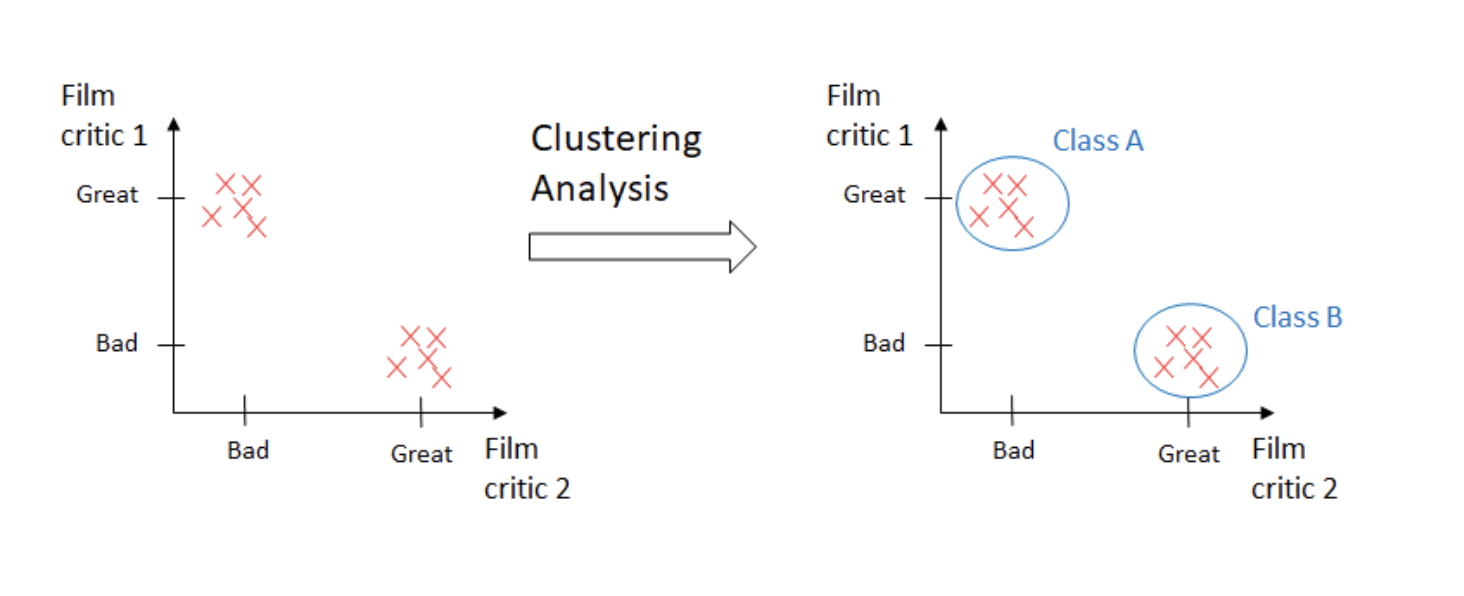
\includegraphics[width=0.85\textwidth]{clustering}
        \end{figure}
        
        Existen muchos algoritmos de clustering que se pueden dividir en dos tipos principales: 
        jerárquicos y particionales.

        \clearpage

        \begin{itemize}
            \item Los algoritmos jerárquicos dividen recursivamente un conjunto de datos en 
            un subconjunto más pequeño hasta que un subconjunto contenga solo un elemento. 
            Esto se puede representar con un dendrograma que se parece a un árbol. 
            
            Se puede construir desde las hojas hasta la raíz (enfoque aglomerativo) o desde la raíz hasta las hojas 
            (enfoque divisivo). En la agrupación jerárquica, no tiene que especificar la cantidad de agrupaciones, 
            sino que debe definir una condición de terminación para el proceso de división / fusión.

            \item Los algoritmos particionales dividen un conjunto de datos en varios subconjuntos 
            (grupos) según un criterio dado. 
            Para algunos algoritmos, el número de grupos debe definirse a priori (por ejemplo, K-Means) y 
            para algunos no (DBSCAN). 
            
            La definición del número de clústeres antes de ejecutar un algoritmo a menudo requiere un conocimiento
            de dominio específico que a menudo es desafiante (o incluso imposible) en muchas aplicaciones. 
            Esto condujo al desarrollo de muchas heurísticas y enfoques simplificados que ayudaron a los 
            analistas sin conocimiento de dominio a elegir el número apropiado de grupos.

            Y si, se que algoritmos como DBSCAN puede verse como otra categoria pero si lo piensas bien, no es mas 
            una subcategoría. 

        \end{itemize}

        Hay una gran cantidad de algoritmos de clustering y actualmente no hay uno solo que domine
        a otros.
        Elegir la mejor depende de la base de datos en sí, un dominio de los datos y los requisitos
        y expectativas del análisis y demás parámetros específicos del problema.

        El objetivo del uso de clusters es identificar patrones o grupos de objetos similares dentro de un
        conjunto de datos de interés.

        Cada grupo contiene observaciones con un perfil similar de acuerdo con un criterio específico. 
        La similitud entre las observaciones se define utilizando algunas medidas de distancia entre observaciones, 
        incluidas las medidas de distancia euclidiana y de correlación.

        Estas son muy usadas en muchos campos, algunos son:
        \begin{itemize}
            \item En la investigación del cáncer, para clasificar a los pacientes en subgrupos según su 
            perfil de expresión génica. Esto puede ser útil para identificar el perfil molecular de 
            pacientes con pronóstico bueno o malo, así como para comprender la enfermedad.
            
            \item 
            En marketing, para la segmentación del mercado mediante la identificación de subgrupos de 
            clientes con perfiles similares y que podrían ser receptivos a una forma particular de publicidad.

            \item 
                En la planificación urbana, para identificar grupos de casas según su tipo, valor y ubicación.
        \end{itemize}

        Como ya vimos la idea de clustering no hace referencia a algoritmos específicos, 
        pero es un proceso para crear grupos basados en medidas de similitud. 
        El análisis de clustering utiliza un algoritmo de aprendizaje no supervisado para crear estos clusters.

        Los algoritmos de clustering generalmente funcionan según el principio simple de maximización 
        de similitudes intragrupo y minimización de similitudes entre grupos. 
        La medida de similitud determina cómo se deben formar los grupos.

        La similitud es una caracterización de la proporción del número de atributos que 
        comparten dos objetos en común en comparación con la lista total de atributos entre ellos. 
        
        Los objetos que tienen todo en común son idénticos y tienen una similitud de 1.0. 
        Los objetos que no tienen nada en común tienen una similitud de 0.0.

        La agrupación se puede adaptar ampliamente en el análisis de las empresas. 
        Por ejemplo, un departamento de marketing puede usar la agrupación para segmentar 
        a los clientes por atributos personales. Como resultado de esto, 
        se pueden diseñar diferentes campañas de marketing dirigidas a varios tipos de clientes.


\part{Segmentación de clientes}

    \chapter{El problema}

        El problema elegido fue el de segmentar clientes en cluster que los representen, buscamos comprender mejor a los
        clientes y brindar información de segmentación para que por ejemplo un equipo de marketing pudiera planificar
        una estrategia efectiva basada en nuestros clusters.

        \section{Importancia de resolverlo / Relevancia}

        Si bien las tácticas de marketing masivo aún pueden obtener resultados (la idea que usa DuckDuckGo), 
        la suposición de que simplemente todos estarán interesados en comprar lo que está vendiendo es una 
        estrategia costosa, ineficiente y una forma bastante mala de tirar dinero de marketing a la basura.

        En lugar de un enfoque de \Quote{talla única}, la segmentación exitosa agrupa los datos de sus 
        clientes en grupos que comparten las mismas propiedades o características de comportamiento, 
        lo que ayuda a impulsar el contenido dinámico y las tácticas de personalización para comunicaciones 
        de marketing más oportunas, relevantes y efectivas (algo como lo que hace Facebook o Google).

        Sin embargo, para que la segmentación se use correctamente, debe tener en cuenta que 
        diferentes clientes compran por diferentes razones, y los especialistas en marketing 
        deben aplicar de manera inteligente una serie de consideraciones que podrían afectar 
        sus decisiones de compra. 
        
        Un profesor de la Harvard Business School incluso llegó a decir que, de 30,000 nuevos lanzamientos 
        de productos de consumo cada año, el 95\% falla debido a la segmentación ineficaz del mercado.

        \cite{3}

    \chapter{El dataset / Business Understanding}

    \section{¿De donde salieron los datos?}
        Para poder solucionar este problema busque un dataset que fuera apropiedo en 
        Kaggle, llegando a este:

        \url{https://www.kaggle.com/vjchoudhary7/customer-segmentation-tutorial-in-python}

        Ahora veamos un poco de contexto de este dataset:

        Este conjunto de datos se creo solo con el propósito de aprender los conceptos de 
        segmentación de clientes, también conocidos como análisis de la carrito de compras :v. 

        Este fue diseñado para usarse con la técnica de ml no supervisada (algoritmo de kmeans) en la forma más simple.
        Es decir es un dataset \Quote{didactico} publicado por el creador de un curso que explicaba kmeans. 

        Este dataset se supone que es de un centro comercial y, a través de tarjetas de membresía, 
        se tienen algunos datos básicos sobre los clientes, como identificación del cliente, 
        edad, sexo, ingresos anuales y puntaje de gastos.

        La puntuación de gasto es algo que asigna al cliente en función de sus parámetros definidos,
        como el comportamiento del cliente y los datos de compra.

        \begin{figure}[ht!]
            \centering
            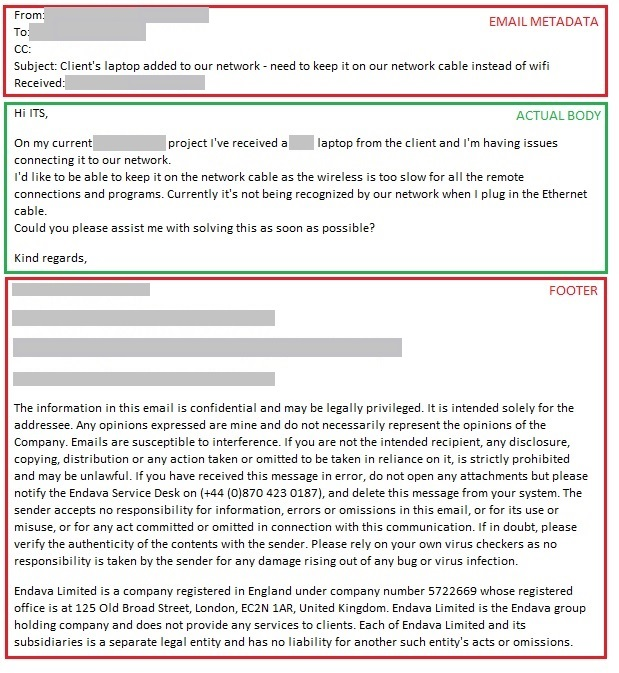
\includegraphics[width=0.7\textwidth]{x}
        \end{figure}

    \chapter{La propuesta}
        Mi hipotesis sería que usando este dataset y 
        mediante aprendizaje no supervisado (kmeans y dbscan) se podría crear un sistema que fuera capaz de clasificar
        a los clientes en un grupos significativos.

        El problema elegido fue el de segmentar clientes en cluster que los representen, buscamos comprender mejor a los
        clientes y brindar información de segmentación para que por ejemplo un equipo de marketing pudiera planificar
        una estrategia efectiva basada en nuestros clusters.

    \chapter{La implementación}

        \section{Preprocesamiento}

            \subsection{Preparación y conocimiento de los datos}

                Lo primero que tuvimos que hacer fue preparar los datos, el primer paso fue descargar el csv y
                abrirlo para explorar un poco
                la naturaleza del dataset.

                \begin{figure}[ht!]
                    \centering
                    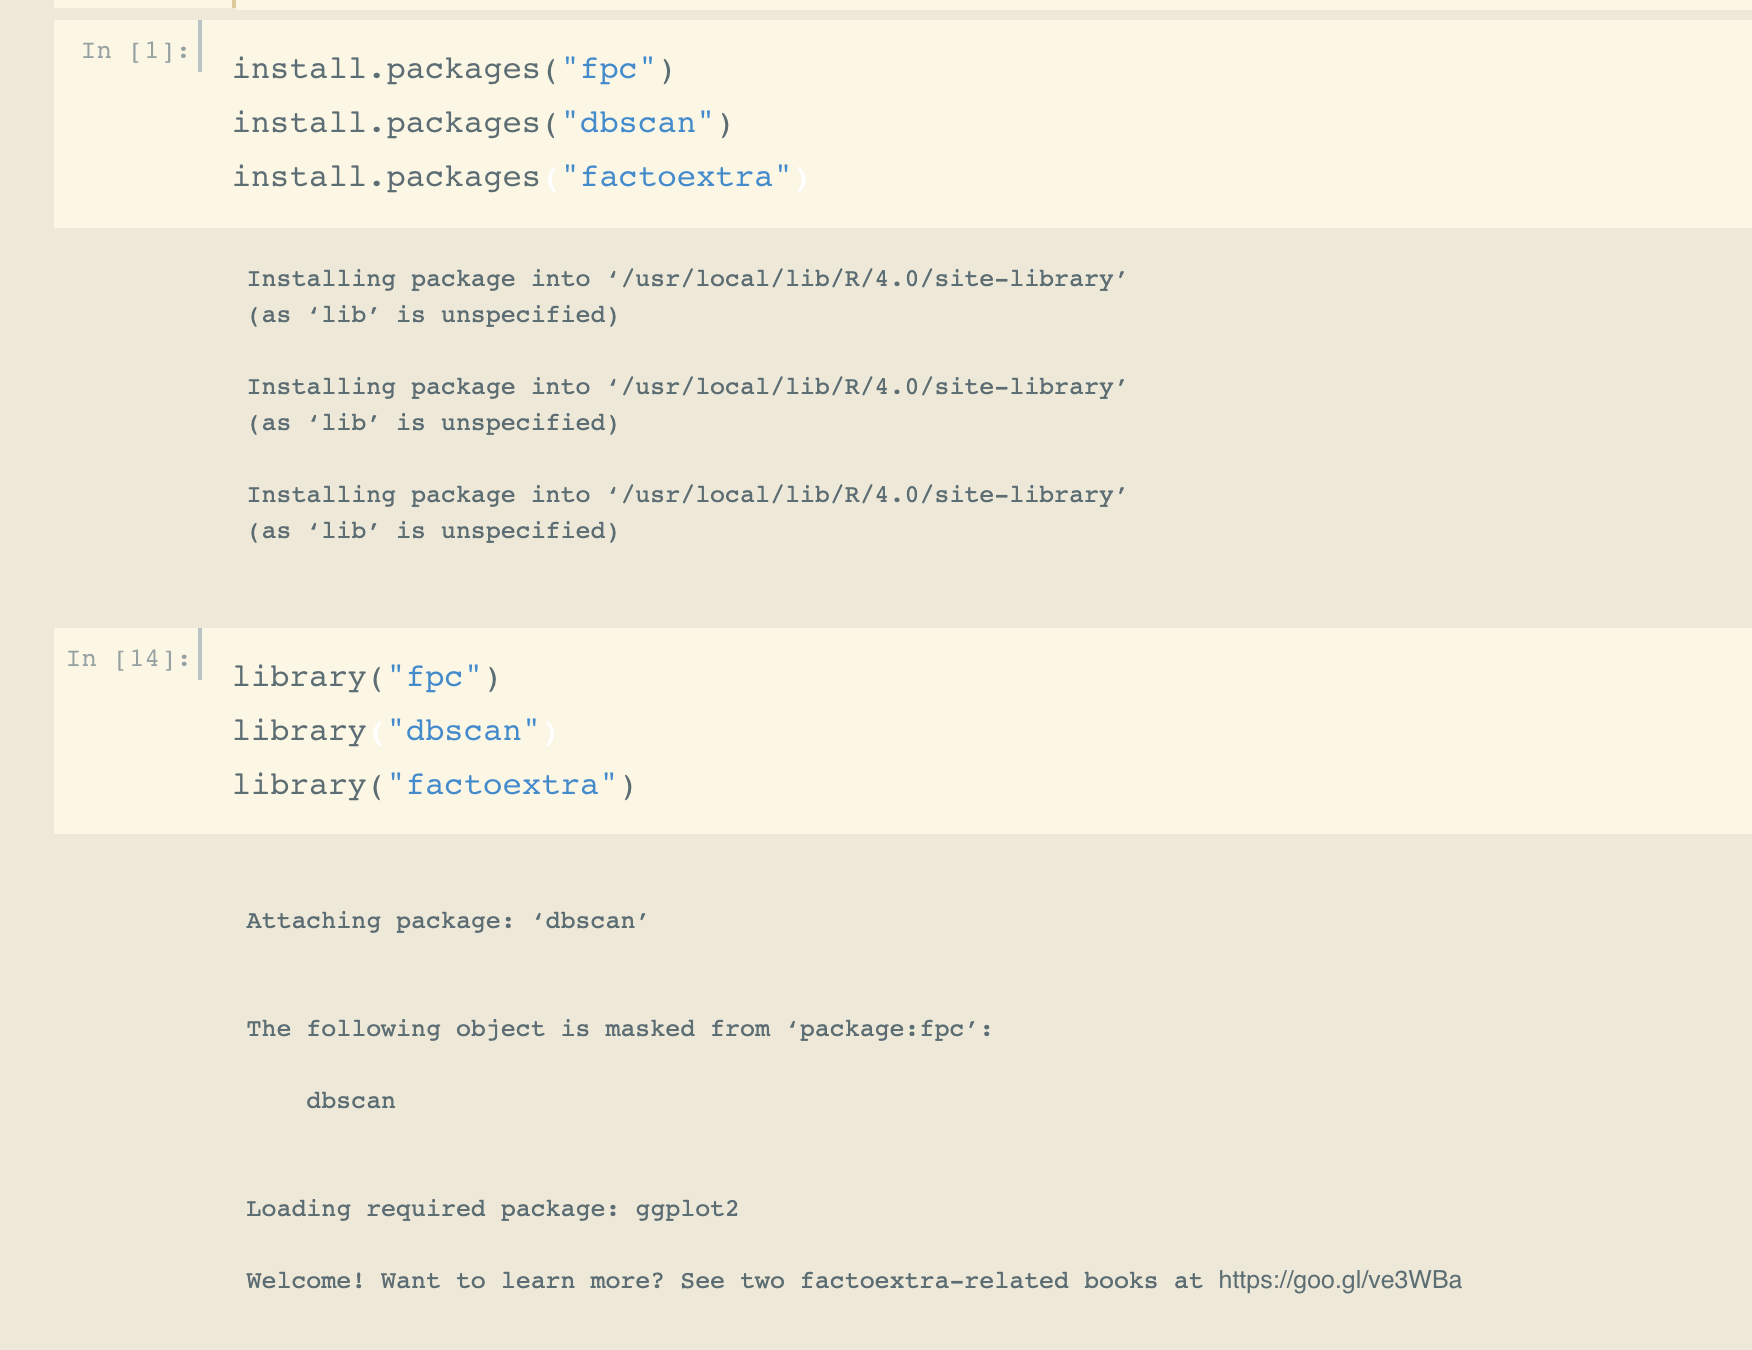
\includegraphics[width=0.8\textwidth]{1}
                    \caption{Primero cargemos las librerias}
                \end{figure}

                \begin{figure}[ht!]
                    \centering
                    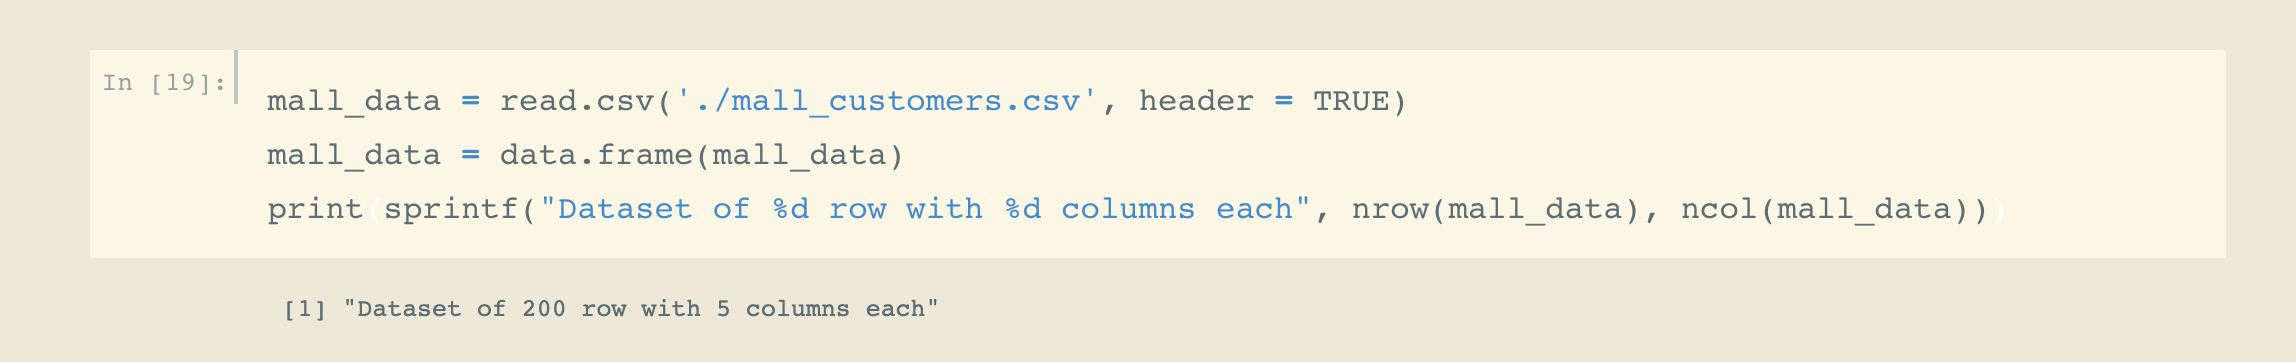
\includegraphics[width=0.8\textwidth]{2}
                    \caption{Leemos la información y la almacenamos en un dataframe}
                \end{figure}

                \begin{figure}[ht!]
                    \centering
                    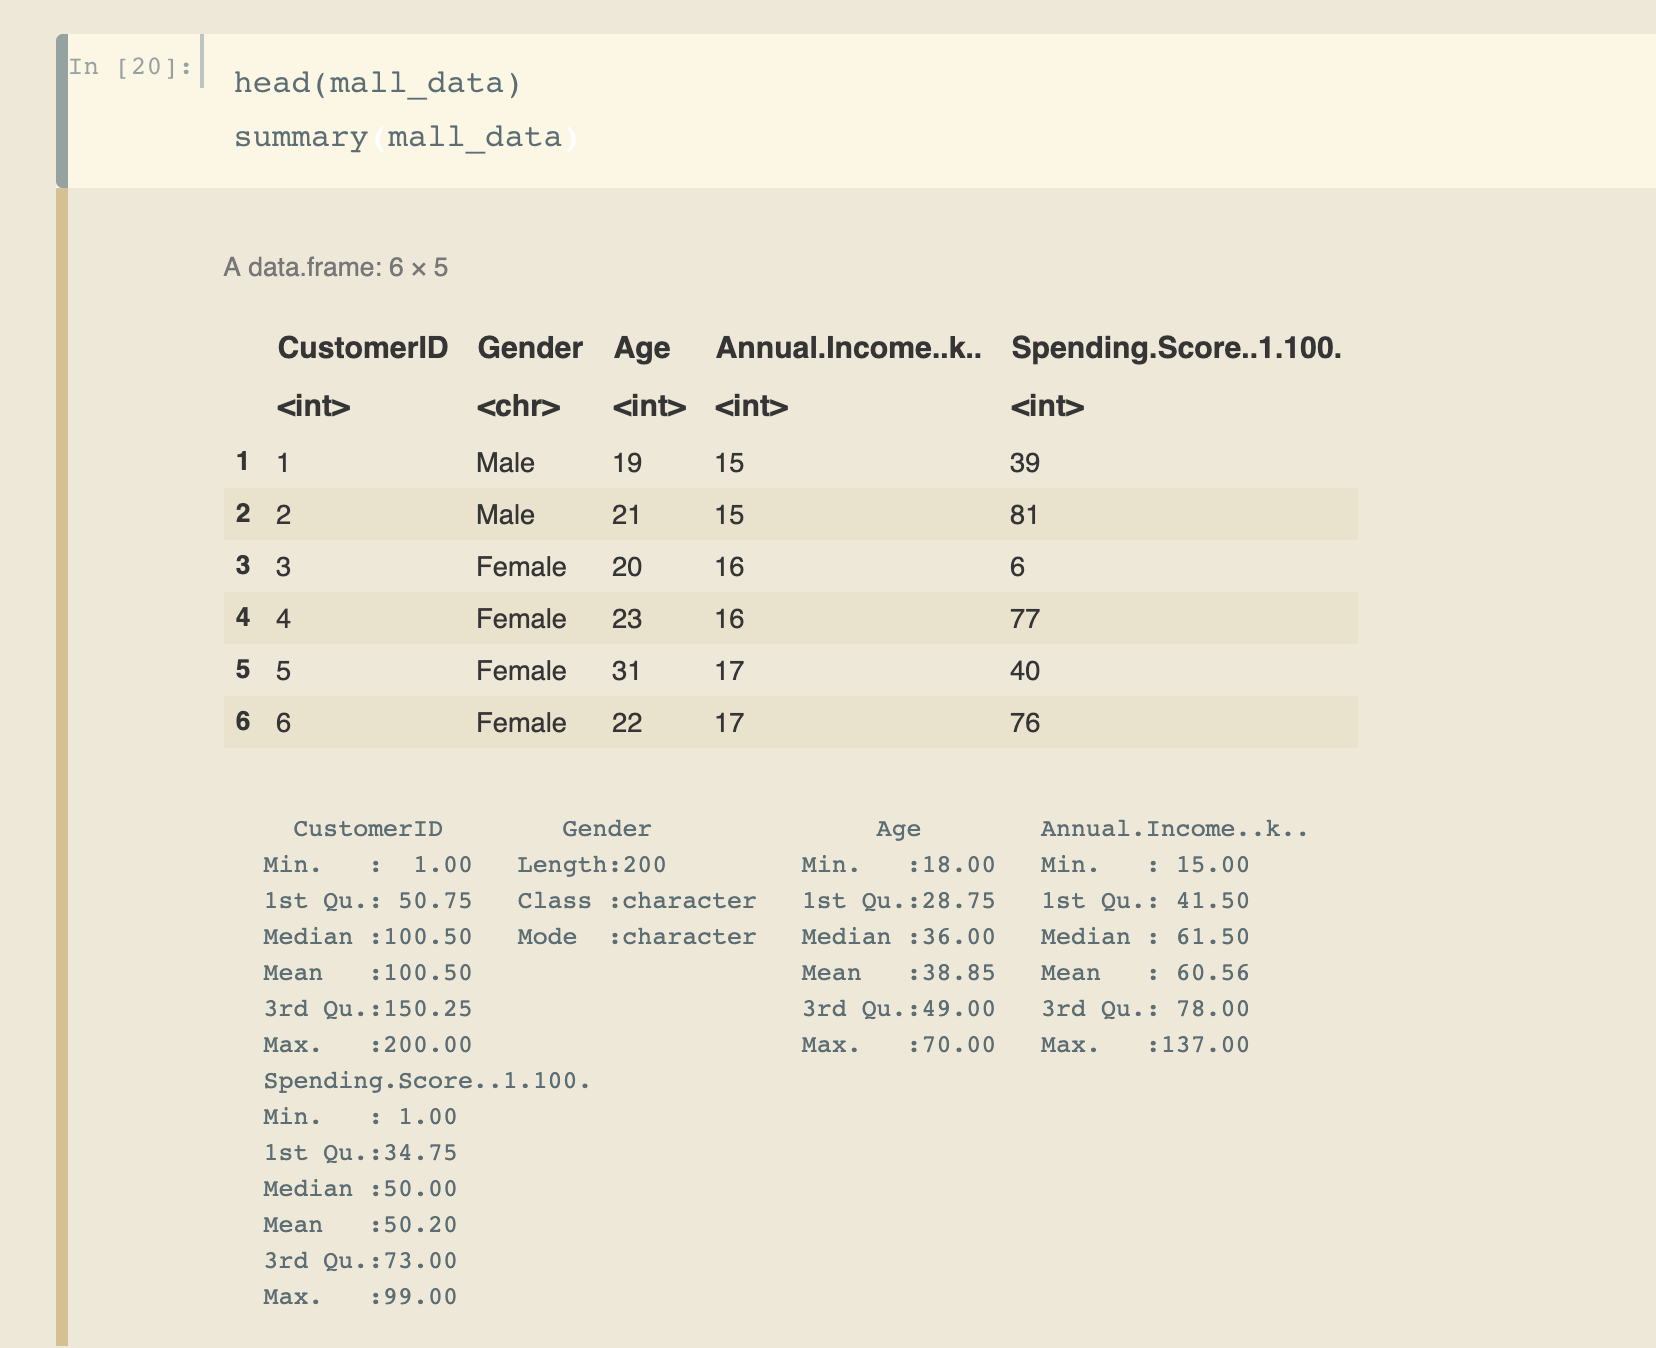
\includegraphics[width=0.8\textwidth]{3}
                    \caption{Usamos las funciones de r para ver un poco mejor el dataset}
                \end{figure}

                \clearpage

            \subsection{Conociendo los datos}

                Hay 5 columnas dentro de nuestra información:

                \begin{itemize}
                    \item ID de cliente: número de cliente numérico único
                    \item Género: categórico, binario (hombre / mujer)
                    \item Edad - numérica, entero
                    \item Ingreso anual (k \$) - numérico, entero
                    \item Puntaje de gasto (1-100) - numérico, entero
                \end{itemize}

            \subsection{Cosa curiosa: usar kmeans sobre columnas binaria}

            Hay una columna binaria, categórica: género.
            Recuerdo haber hablado con el profesor sobre que era una mala idea usar un numero para poner esa columna
            (por ejemplo hombre 1 y mujer 0), despues de eso pense en usar algo parecido al one hot encoding.
            
            Y llegue a esta conclusion:
            \begin{itemize}
                \item técnicamente posible
                \item teóricamente no prohibido
                \item prácticamente no recomendado
            \end{itemize}
                
            Por qué no se recomienda, se explica muy bien en el sitio de soporte de IBM. 

            \url{https://www.ibm.com/support/pages/clustering-binary-data-k-means-should-be-avoided}


            \subsection{Limpieza de datos}
                
            \textbf{No hay datos faltantes. 
                Esto simplifica el análisis, pero es un escenario muy poco probable
                en la vida real, donde los científicos de datos se pueden pasan una cantidad significativa de
                tiempo limpiando
                sus datos antes de realizar el análisis central.}

                \clearpage
                
                Eso si, es importante notar que para que todo funcione en los algoritmos que usaremos después
                vamos a quedarnos solo con las columnas numéricas, es decir, adiós el género como un dato categorico
                y al solo ser binario podemos usar valores numéricos.

                \begin{figure}[ht!]
                    \centering
                    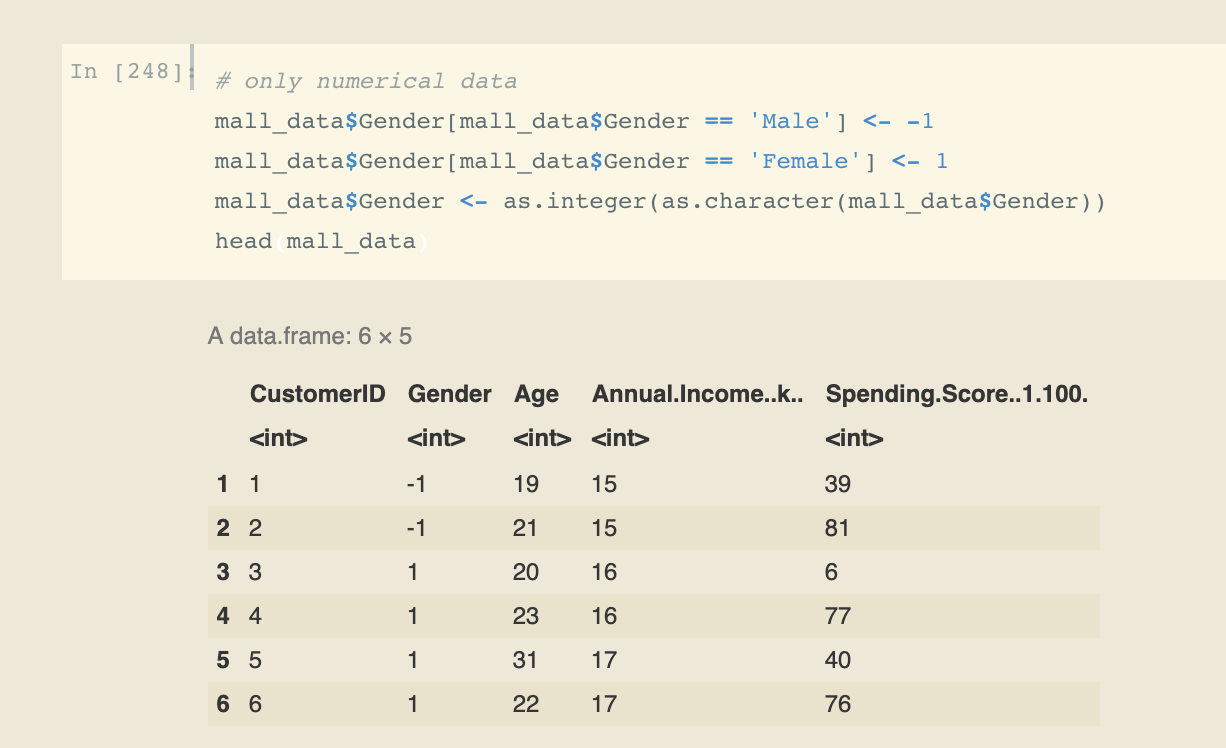
\includegraphics[width=0.8\textwidth]{miss}
                \end{figure}

        \clearpage
        \section{Exploración de datos}

            Esta sección contiene una investigación estadística básica de una base de datos dada. 
            Es un punto crucial en cualquier análisis, ya que permite una mejor comprensión de los datos.

            Los datos los voy a separar por género, la única variable categórica.

            \subsection{Edades}

                \begin{figure}[ht!]
                    \centering
                    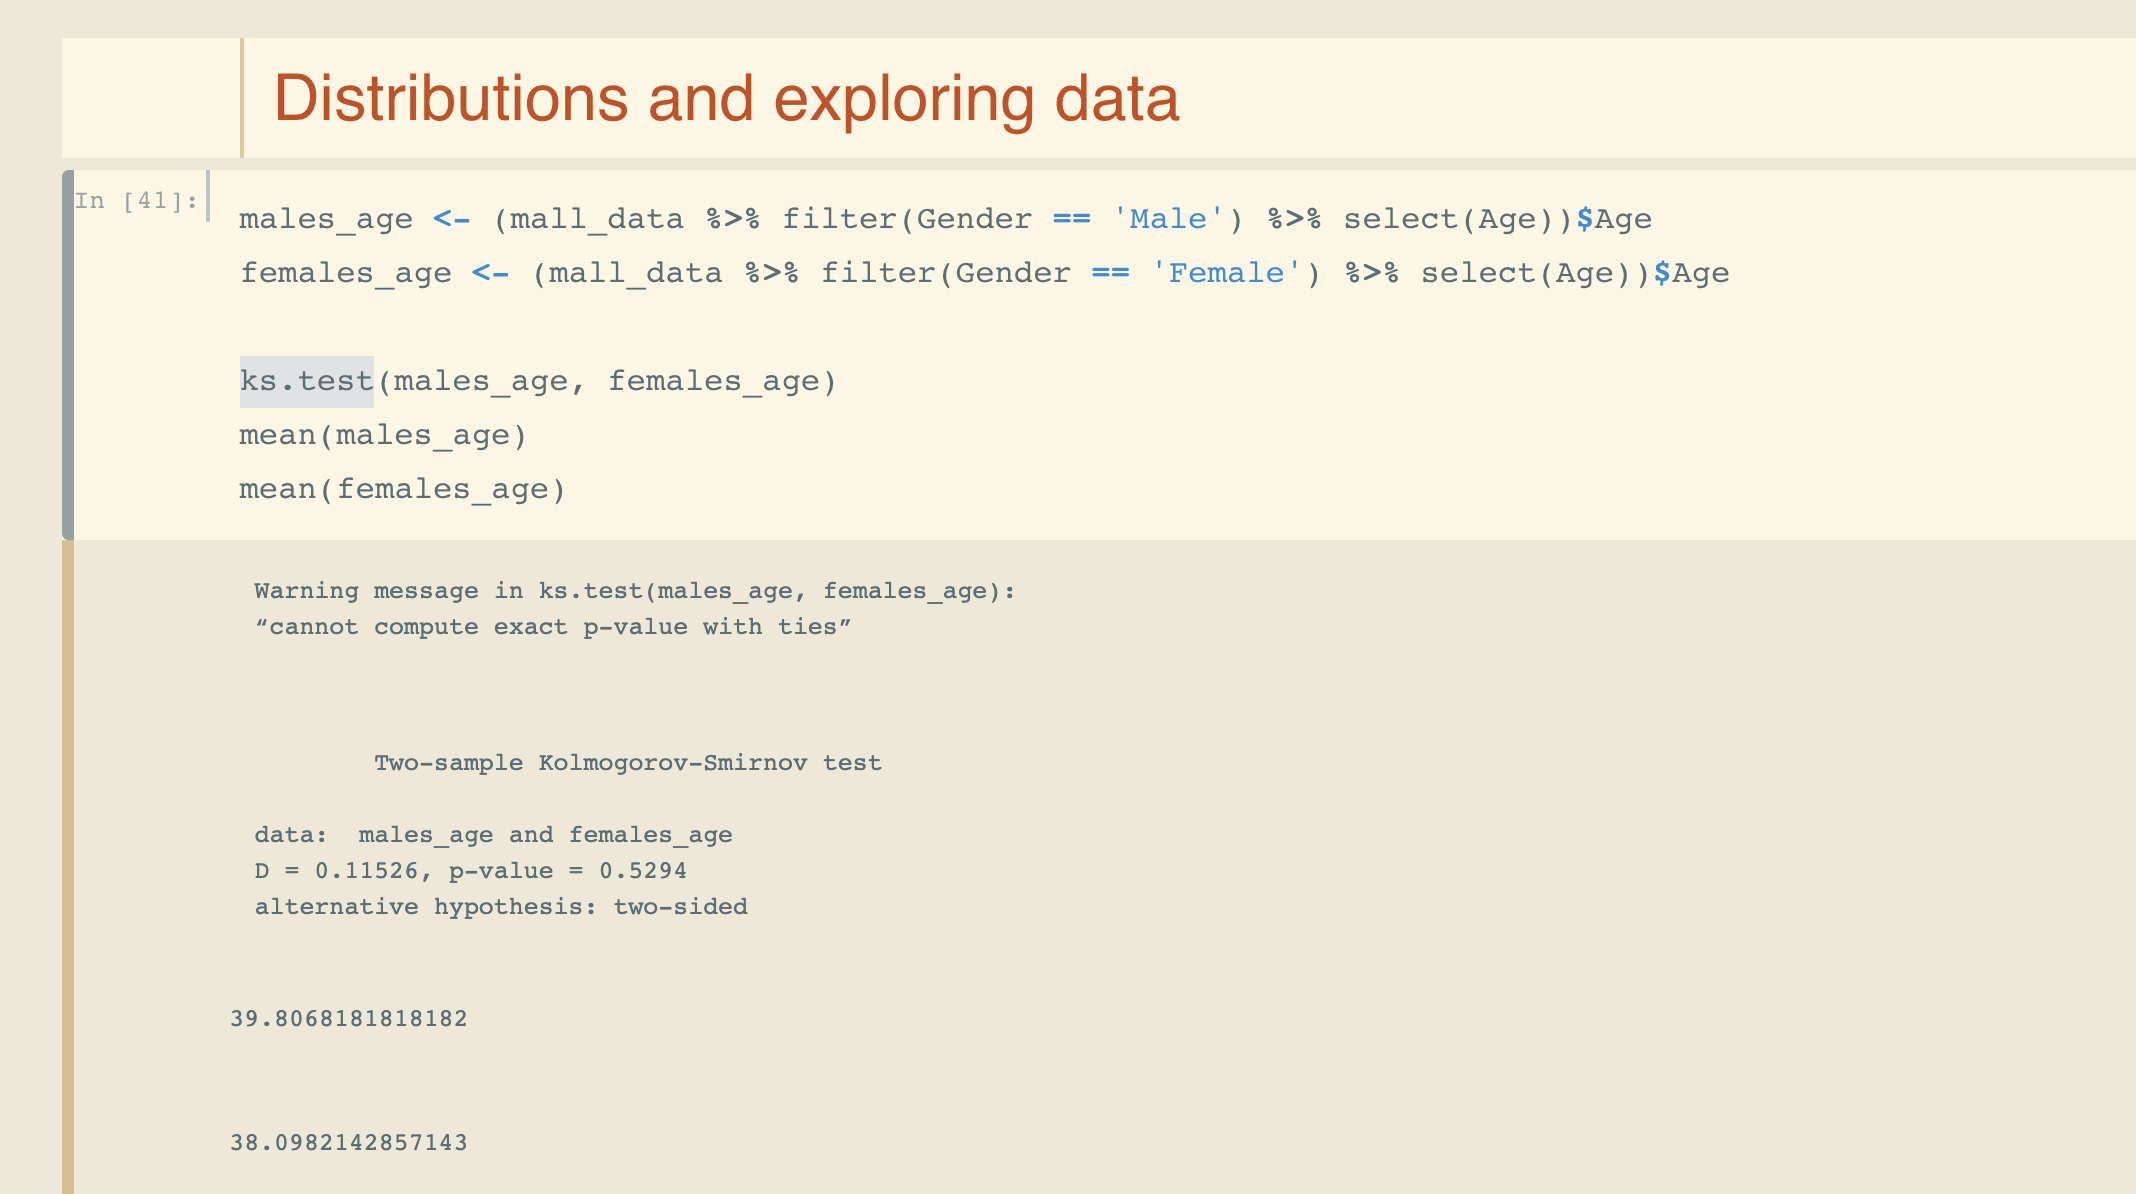
\includegraphics[width=0.8\textwidth]{4}
                \end{figure}

                \begin{figure}[ht!]
                    \centering
                    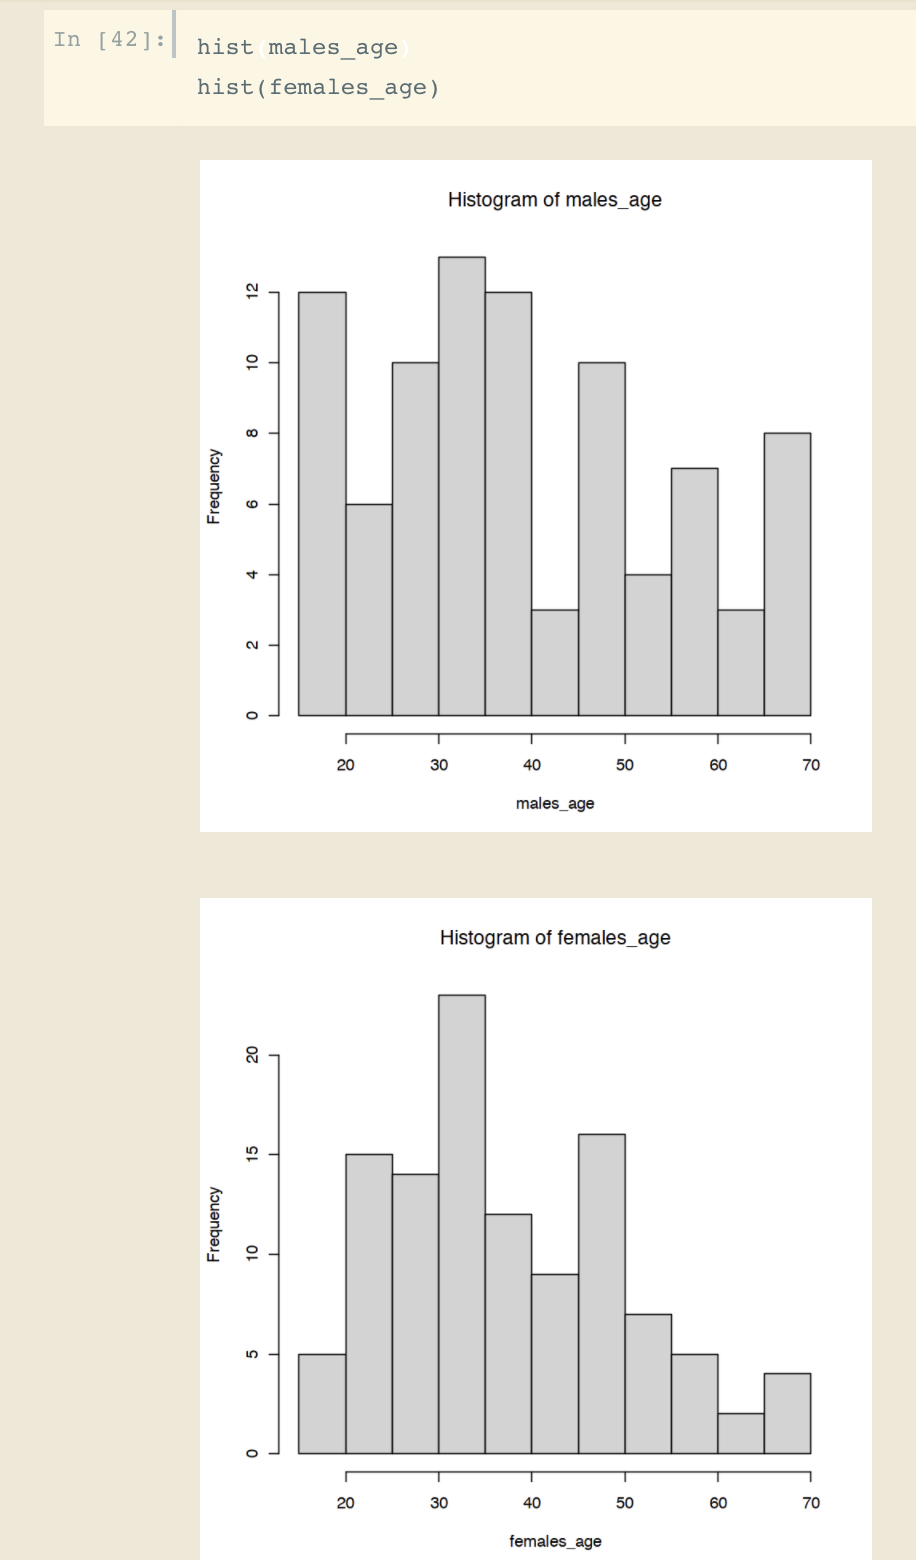
\includegraphics[width=0.3\textwidth]{5}
                \end{figure}

                La edad promedio de los clientes masculinos es ligeramente más
                alta que la de las mujeres (39.8 versus 38.1). La distribución de 
                la edad masculina es más uniforme que la femenina, donde podemos
                observar que el grupo de edad más grande es de 30 a 35 años. 
                
                Sin embargo, la prueba K-S muestra que las diferencias entre estos 
                dos grupos son estadísticamente insignificantes.

                Aquí hay un poco más de clientes femeninos que masculinos (112 vs. 88). 
                Las mujeres representan el 56\% del total de clientes.

                \begin{figure}[ht!]
                    \centering
                    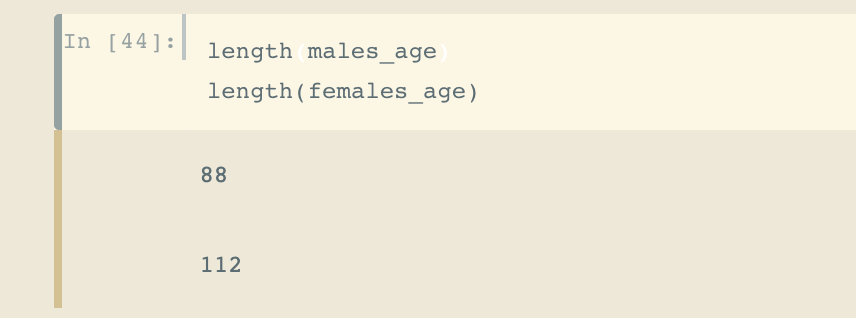
\includegraphics[width=0.5\textwidth]{6}
                \end{figure}

            \clearpage
            \subsection{Ingresos}

                El ingreso promedio de los hombres es mayor que el de las mujeres (62.2k \$ vs. 59.2k \$). 
                También el ingreso medio de los clientes masculinos (62.5k \$) es mayor que el de las mujeres (60k \$). 
                
                La desviación estándar es similar para ambos grupos. Hay un valor atípico en el grupo masculino con un ingreso anual
                de aproximadamente 140k \$. La prueba K-S muestra que estos dos grupos no son estadísticamente diferentes.

                \begin{figure}[ht!]
                    \centering
                    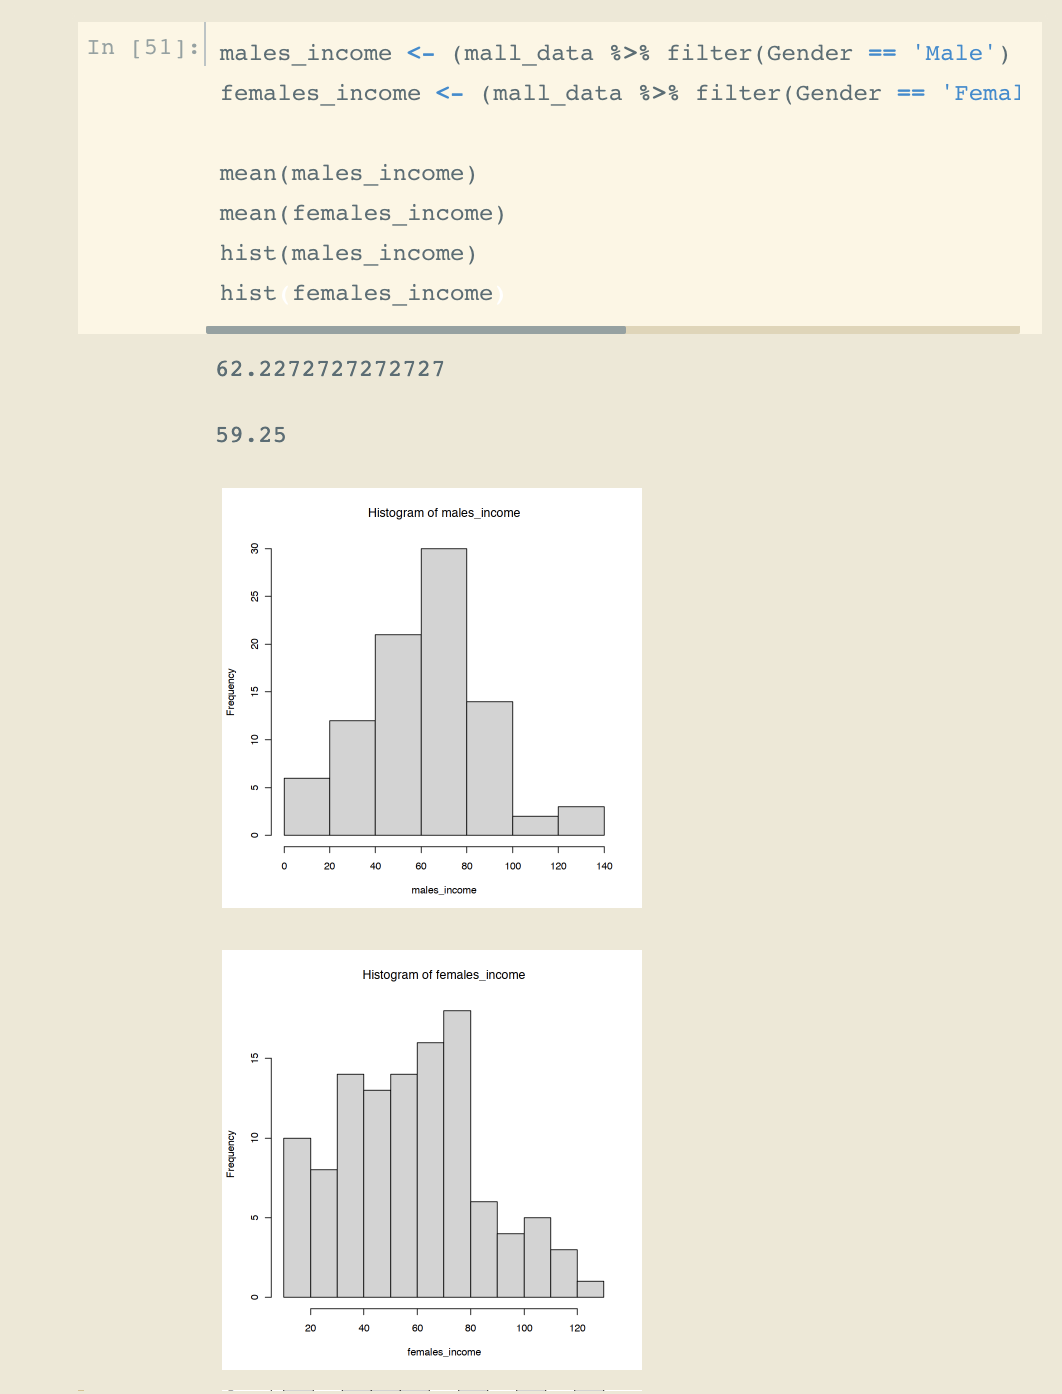
\includegraphics[width=0.5\textwidth]{7}
                \end{figure}

            \clearpage
            \subsection{Gasto}

                Elgasto promedio para las mujeres (51.5) es más alto que el de los hombres (48.5). 
                El valor p de la prueba K-S indica que no hay evidencia para rechazar la hipótesis nula, 
                sin embargo, la evidencia no es tan fuerte como en comparaciones anteriores.

                \begin{figure}[ht!]
                    \centering
                    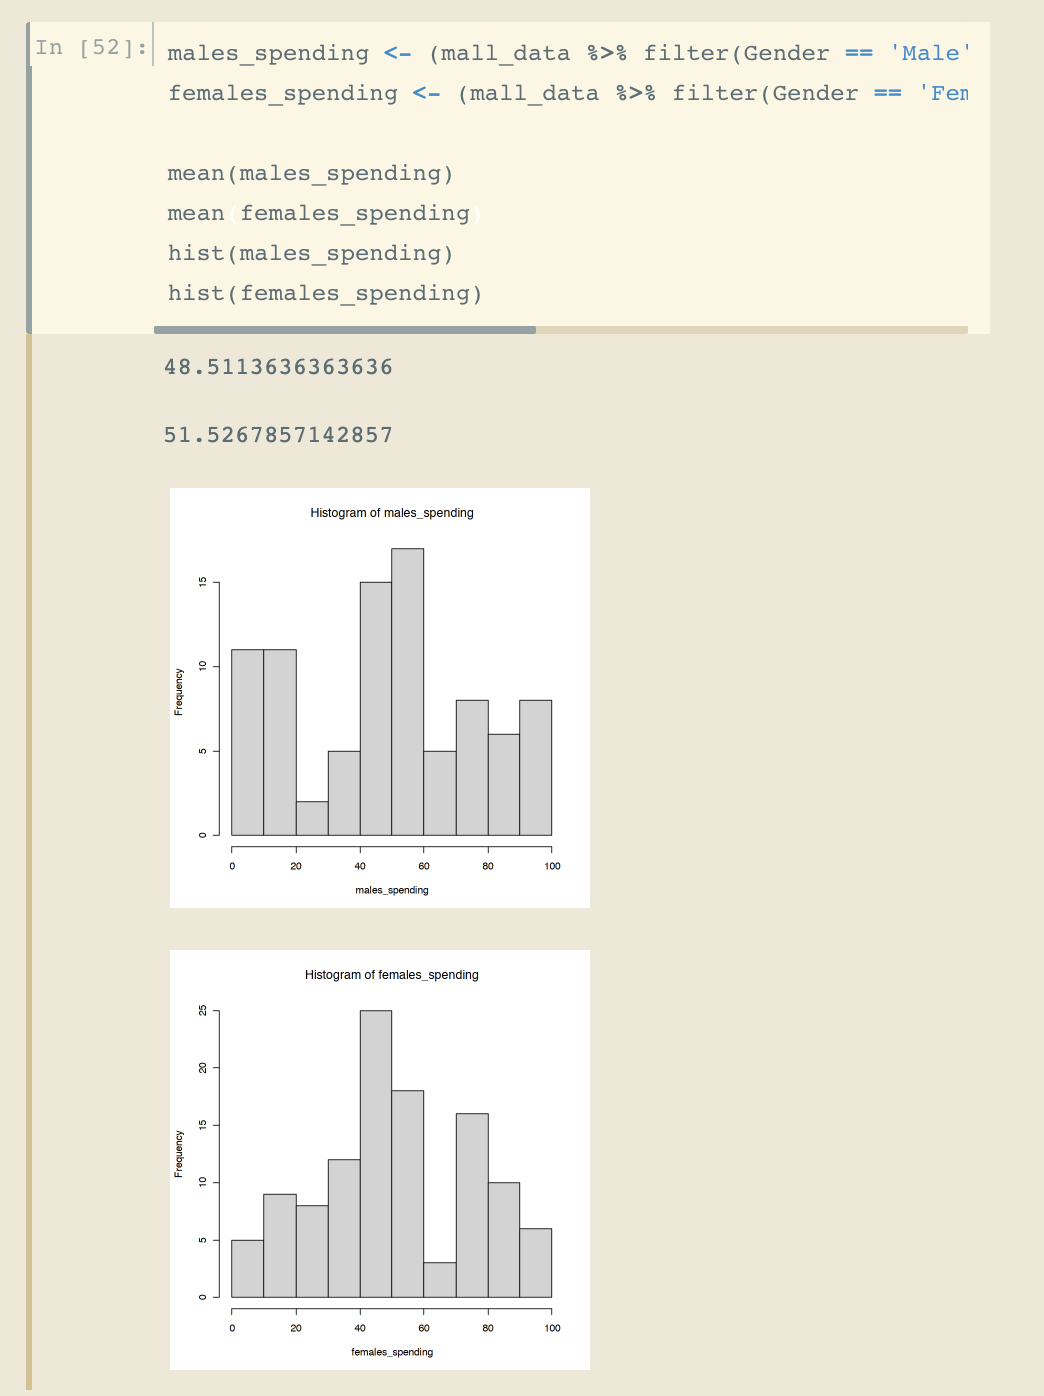
\includegraphics[width=0.5\textwidth]{8}
                \end{figure}

            \clearpage
            \subsection{Posibles correlaciones que no encontre}

                \begin{figure}[ht!]
                    \centering
                    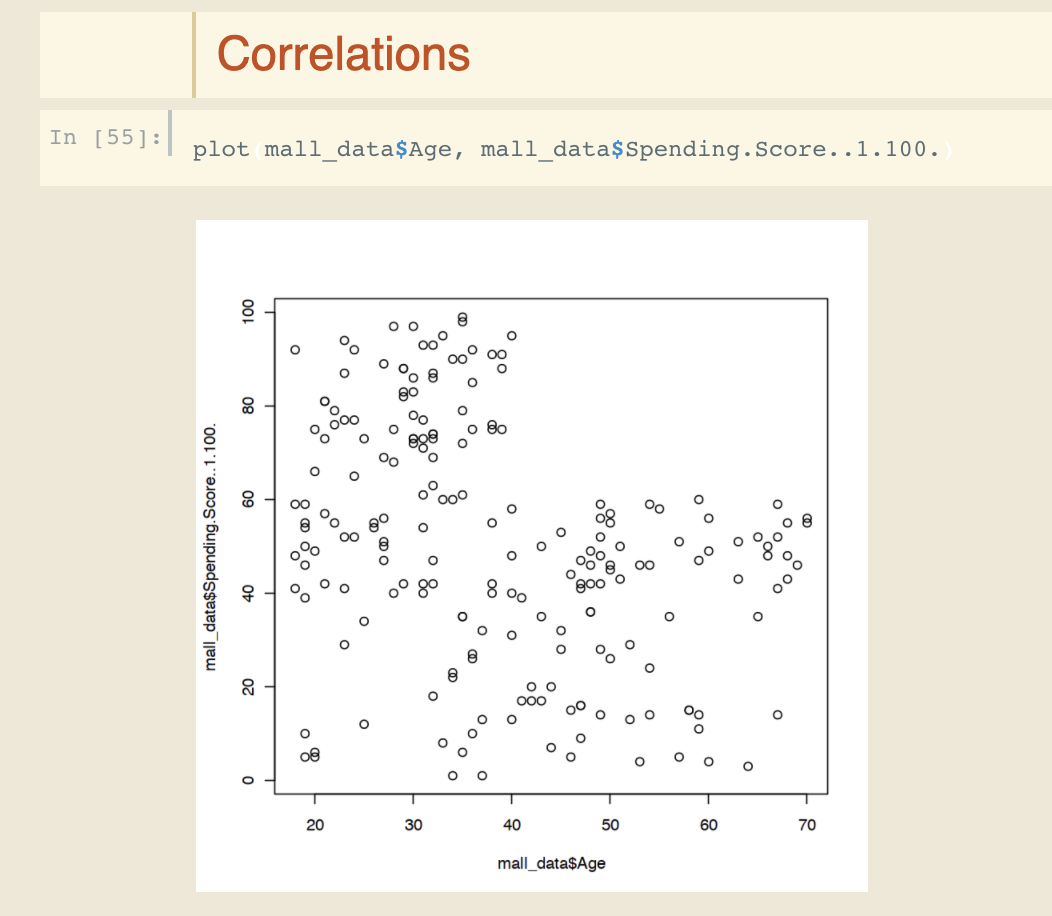
\includegraphics[width=0.5\textwidth]{9}
                    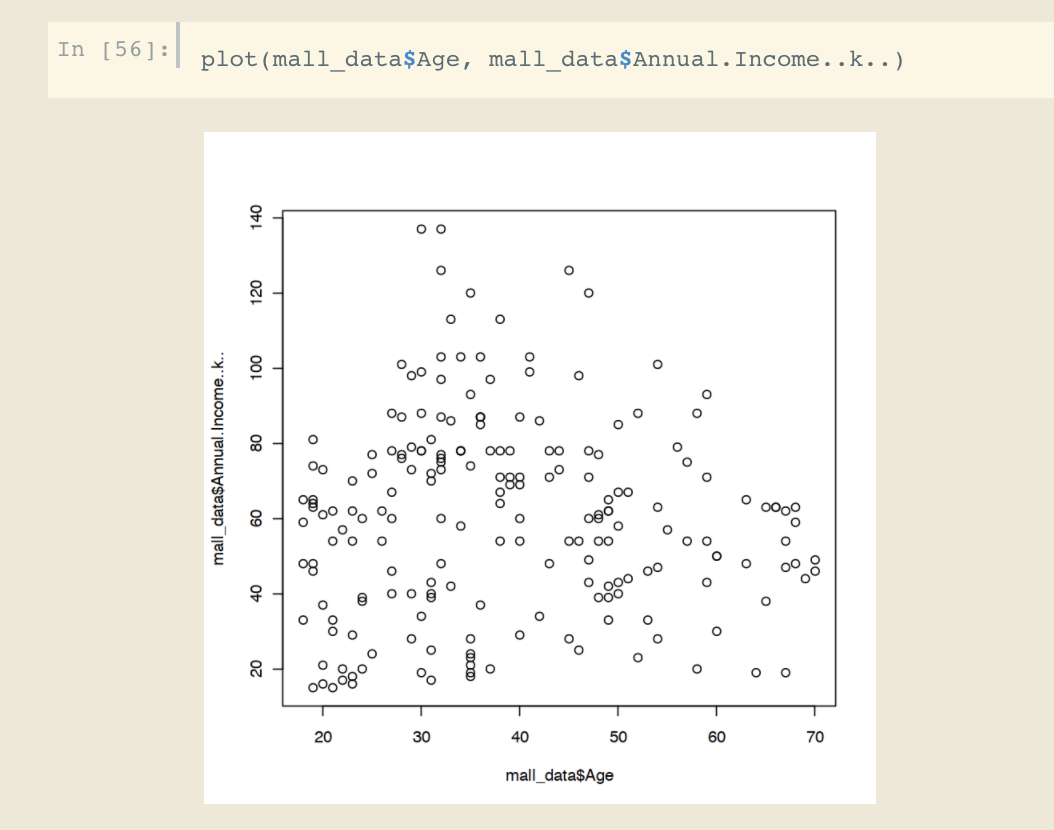
\includegraphics[width=0.5\textwidth]{91}
                    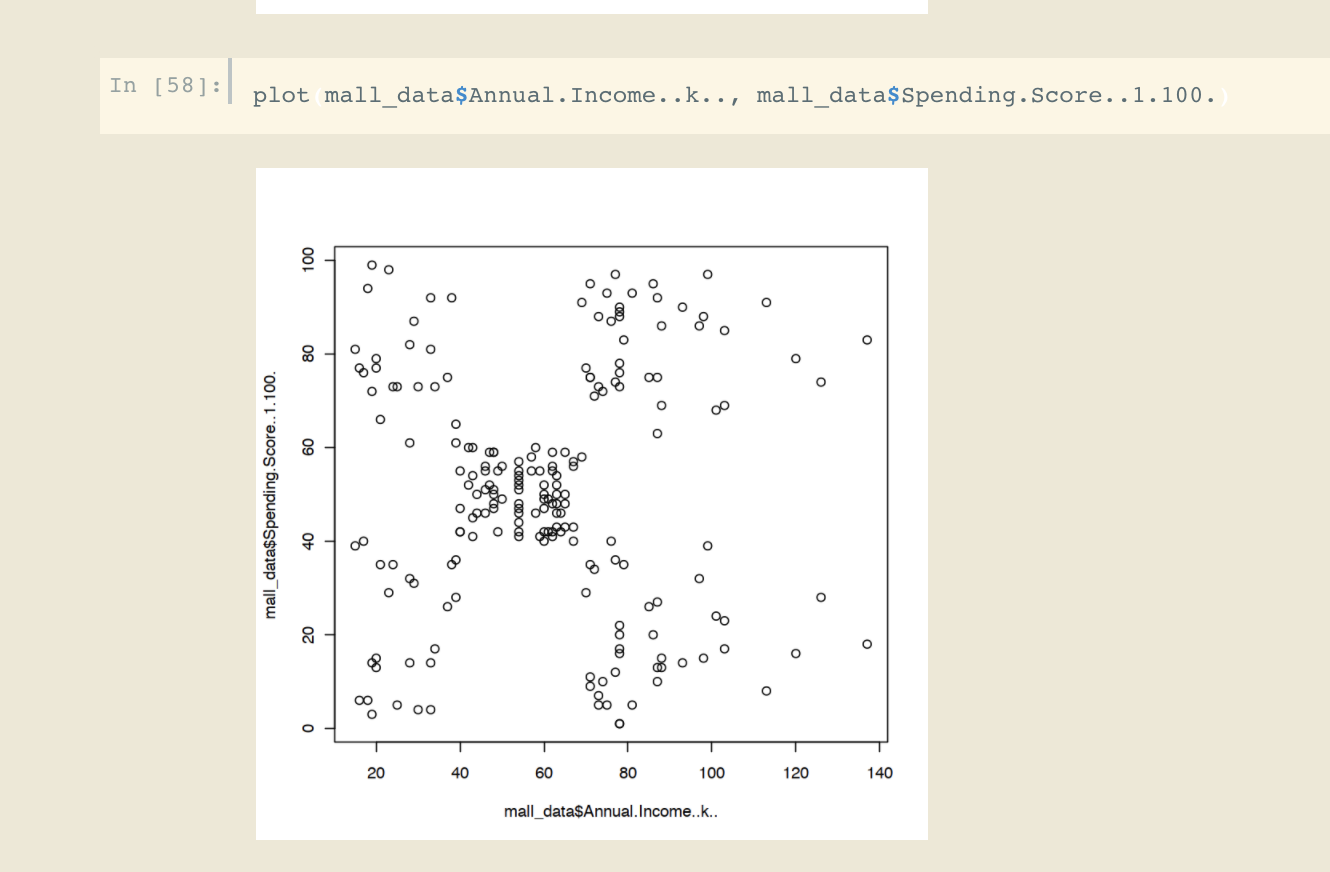
\includegraphics[width=0.5\textwidth]{92}
                \end{figure}

            Volvamos un poco atras y hablemos de los clasificadores que vamos a usar:

    \clearpage
    \section{Técnica: K means}
        \subsection{Historia y funcionamiento}
        La agrupación particional (o agrupación de partición) son métodos de agrupación 
        utilizados para clasificar los elementos dentro de un conjunto de datos en múltiples grupos en función de su similitud. 
        Los algoritmos requieren que el analista especifique el número de clústeres que se generarán.

        K-Means, el algoritmo por excelencia de clustering, muy popular y el que se enseña en la mayoría de los cursos de aprendizaje automático.
        
        Es ademas un algoritmo de agrupación particional.
        Fue desarrollado independientemente en muchos lugares en los años 50 y 60 y ganó gran popularidad debido a su 
        facilidad de implementación, simplicidad y muchos éxitos empíricos (por ejemplo, en negocios, medicina y ciencia).

        Hay 3 pasos principales en el algoritmo K-Means (también conocido como algoritmo de Lloyd):
        \begin{itemize}
            \item Dividir las muestras en grupos iniciales mediante el uso de puntos de semillas. Las muestras más cercanas a estos puntos de origen crearán grupos iniciales.
            \item Calcule las distancias de las muestras a los puntos centrales de los grupos (centroides) y asigne las muestras más cercanas a su grupo.
            \item El tercer paso es calcular los centroides de clúster recién creados (actualizados).
        \end{itemize}

        Luego simplemente hay que repetir los pasos 2 y 3 hasta que el algoritmo converja.
        Como se mencionó anteriormente, el objetivo de K-Means es minimizar la función objetivo (inercia) 
        en todos los grupos. 
        
        La función objetivo comunmene esta definida como:
        \begin{figure}[ht!]
            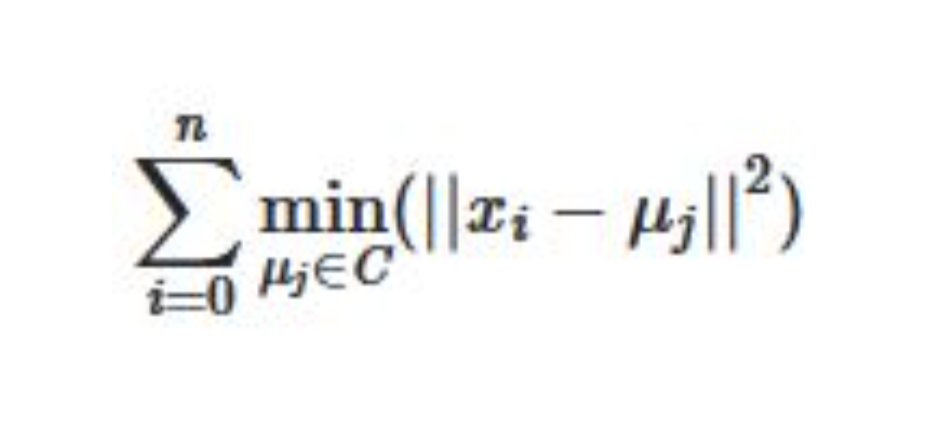
\includegraphics[width=0.3\textwidth]{min}
        \end{figure}

        Esto se conoce como problema NP-fuerte, lo que significa que es un algoritmo greeady y converge al mínimo local. 
        El costo computacional del algoritmo K-Means de Lloyd es O (kn), donde k es una cantidad de grupos y n es una cantidad de muestras. 

        Esto no es malo en comparación con otros algoritmos de agrupación. A pesar de converger generalmente a un mínimo local, K-means.
        es relativamente rápido y cuando los grupos están bien aislados unos de otros, 
        es probable que converga al mínimo global. Debido a que el resultado de la agrupación depende de los criterios de inicialización, 
        es común ejecutar el análisis para varios puntos de inicialización y elegir el que tenga la mínima inercia resultante.
            
        Hay algunas
        mejoras en el algoritmo para resolver el problema de los mínimos locales. Una mejora ejemplar es utilizar 
        algoritmos mejorados de Firefly.

        Esto se conoce como problema NP-hard, lo que significa que es un algoritmo codicioso y converge al mínimo local. El costo computacional del algoritmo K-Means de Lloyd es O (kn), donde k es una cantidad de grupos yn es una cantidad de muestras. Esto no es malo en comparación con otros algoritmos de agrupación. A pesar de converger generalmente a un mínimo local, K-means es relativamente rápido y cuando los grupos están bien aislados unos de otros, es probable que converja al mínimo global. Debido a que el resultado de la agrupación depende de los criterios de inicialización, es común ejecutar el análisis para varios puntos de inicialización y elegir el que tenga la mínima inercia resultante. Hay algunas mejoras en el algoritmo para resolver el problema de los mínimos locales. Una mejora ejemplar es utilizar Algoritmos mejorados de Firefly sobre los cuales puede leer aquí.

        En general, se requiere definir tres parámetros principales:

        \begin{itemize}
            \item Criterios de inicialización
            
            En muchas librerias, se implementa un ingenioso esquema de 
            inicialización: "k-means ++" propuesto por Arthur y Vassilvitskii. 
            
            Crea centroides iniciales generalmente distantes entre sí, lo que aumenta la 
            probabilidad de obtener mejores resultados. 
            También existe la posibilidad de utilizar un generador de puntos aleatorios. 
            Hay esfuerzos continuos para crear el método de siembra más eficiente para el algoritmo K-Means,
                uno de ellos se basa en el análisis de componentes independientes.

            \item 
                Numero de clusters

                La selección de varios grupos es la parte más difícil de configurar este algoritmo. 
                No existen criterios matemáticos estrictos para esto y se han desarrollado muchos enfoques heurísticos / simplificados. 
                Uno de los más simples y populares es el método de codo que se muestra en este análisis.
                
                También hay otras opciones, a menudo avanzadas, para elegir la cantidad óptima de clústeres, por ejemplo:
                \begin{itemize}
                    \item Longitud mínima del mensaje (MML)
                    \item Longitud mínima de descripción (MDL)
                    \item Criterio de información de Bayers (BIC)
                    \item Criterio de información de Akiake (AIC)
                    \item Proceso de Dirichlet
                    \item Estadísticas de brecha
                \end{itemize}

            \item Una métrica de distancia (no se requiere en la implementación)
            
                Hay varias opciones para calcular la distancia entre puntos.
                La más popular es simplemente la métrica euclidiana y es la implementada en R. 
                A menudo se le llama modelo esférico de k-medias. Tiene el inconveniente de que solo encuentra grupos
                de tipo esférico y tiende a inflarse en análisis altamente multidimensionales ("maldición de la dimensionalidad"). 
                Hay otras opciones pero no implementadas en R por defecto, por ejemplo:
                \begin{itemize}
                    \item Distancia de Mahalonobis (alto costo de cómputo)
                    \item Distancia Itakura-Saito
                    \item L1 distancia
                    \item Distancia coseno
                    \item Distancia de Bregman
                \end{itemize}
        \end{itemize}

        Algunas conclusiones sobre K-Means:
        \begin{itemize}
            \item Se utilizan distancias euclidianas
            \item Se debe definir el número de grupos para el algoritmo
            \item El centroide se calcula utilizando la distancia media a los miembros del grupo
            \item Los grupos se suponen isotrópicos y convexos.
            \item Algoritmo estocástico: los resultados dependen de los criterios de inicialización
            \item Crea grupos de igual varianza (minimiza la inercia)
            \item Propenso a la "maldición de la dimensionalidad"
            \item Se puede ejecutar en paralelo, por lo que se escala bien
        \end{itemize}

        \subsection{Ventajas y desventajas}

            K-means es uno de los métodos de clustering más utilizados. 
            Destaca por la sencillez y velocidad de su algoritmo, sin embargo, presenta una serie de
                limitaciones que se deben tener en cuenta.

            Requiere que se ponga de antemano el número de clusters que se van a crear. Esto puede ser 
            complicado si no se tiene la información adicional sobre los datos con los que se trabaja. 
            Se han desarrollado varias estrategias para ayudar a identificar potenciales valores óptimos de K 
            (ver más adelante), aunque todas ellas son orientativas.

            Las grupos resultantes pueden variar dependiendo de la asignación aleatoria inicial de los 
            centroides. Para minimizar este problema se recomienda repetir el proceso de clustering entre 25-50 
            veces y seleccionar como resultado definitivo el que tenga menor suma total de varianza interna. 
            Aun así, solo se puede garantizar la reproducibilidad de los resultados si se emplean semillas.

            Presenta problemas de robustez frente a outliers. La única solución es excluirlos o recurrir a 
            otros métodos de clustering más robustos como K-medoids (PAM).


        \clearpage
        \subsection{Apliquemoslo a los datos}

        \subsubsection{¿Qué parametros usar?}


            Para encontrar un número apropiado de clusters, se utilizará una metrica bastante conocida, la del codo:
            \begin{figure}[ht!]
                \centering
                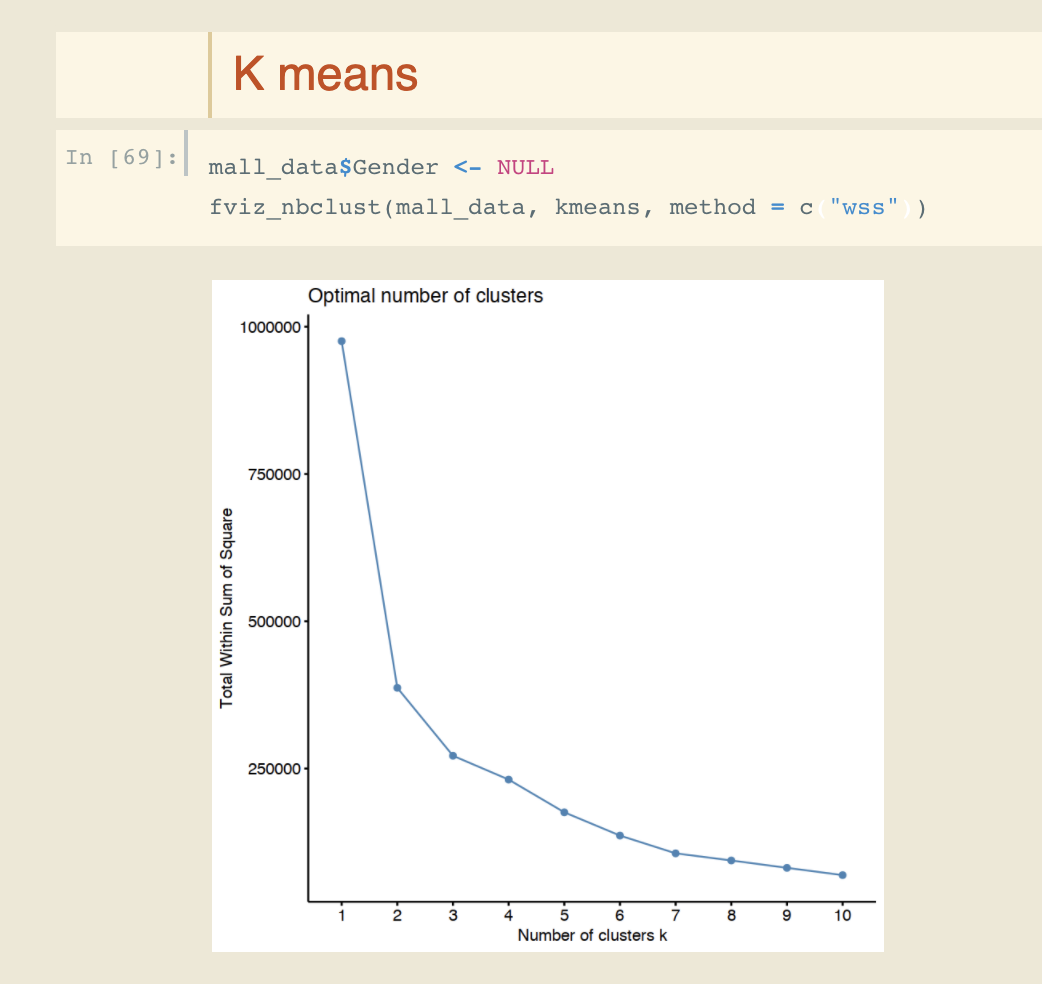
\includegraphics[width=0.75\textwidth]{k1}
            \end{figure}

            Esta de una resultado entre el 5 y el 6, asi que intentaremos con ambos para ver.

            \begin{figure}[ht!]
                \centering
                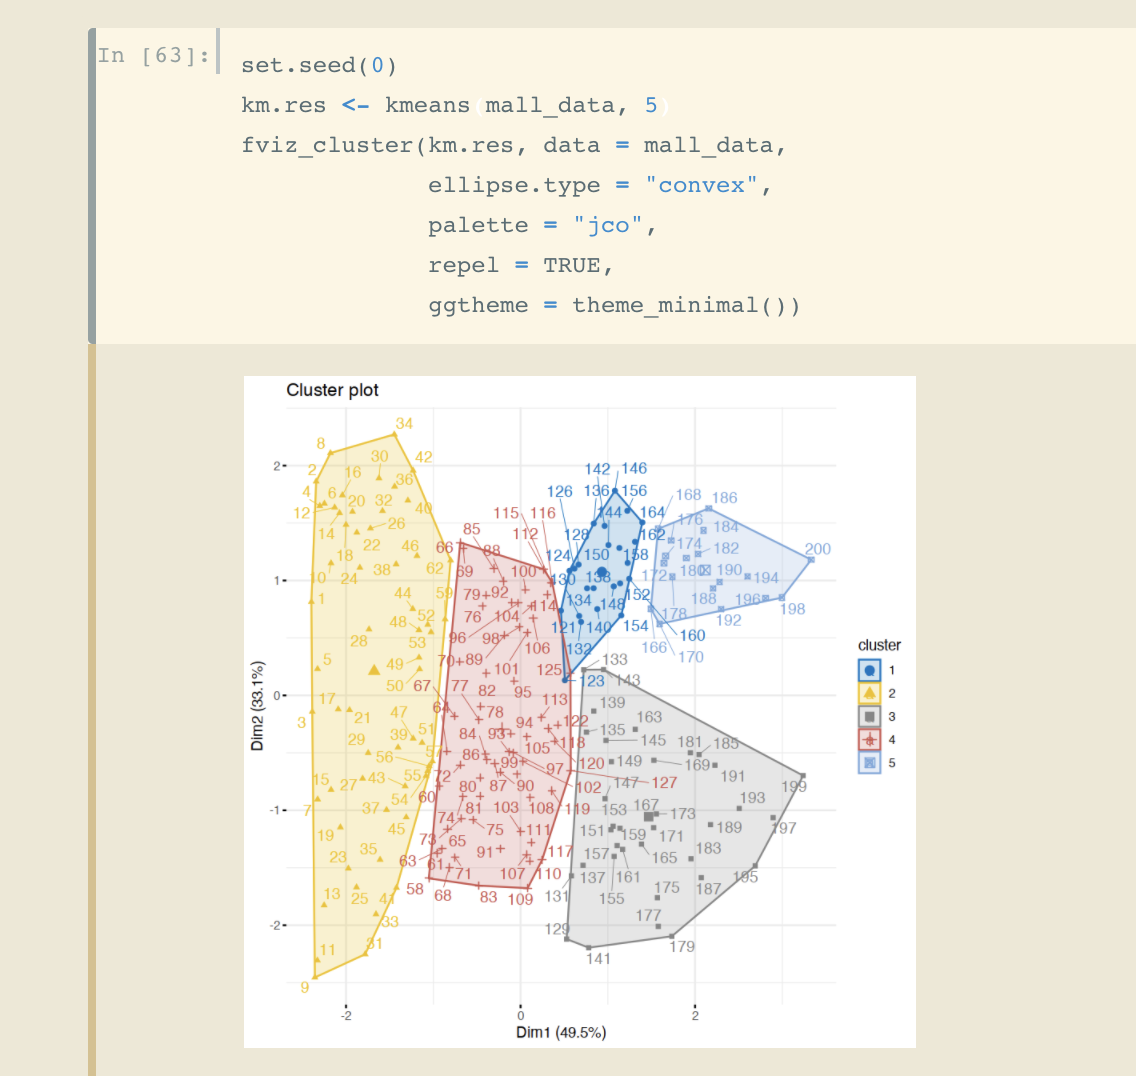
\includegraphics[width=0.8\textwidth]{k2}
                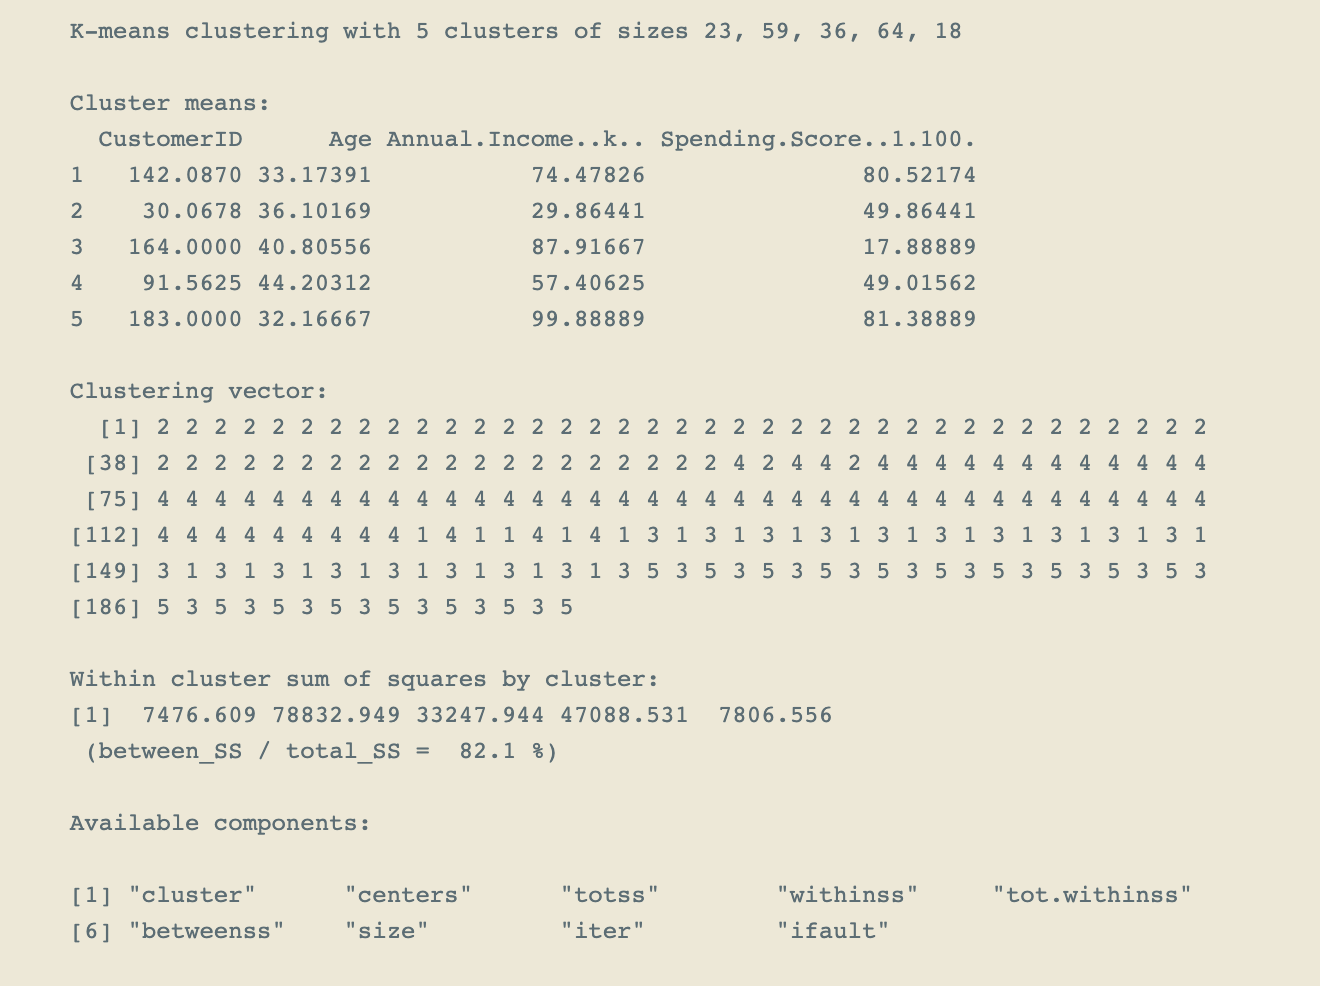
\includegraphics[width=0.8\textwidth]{k21}
            \end{figure}

            \subsubsection{Para 5 paso esto:}

            El algoritmo K-Means generó los siguientes 5 grupos:

            \begin{itemize}
                \item clientes con bajo  ingreso anual y  alto  puntaje de gasto
                \item clientes con ingreso  medio  y  puntaje de gasto  medio
                \item clientes con alto  ingreso anual y  bajo  puntaje de gasto
                \item clientes con altos  ingresos anuales y  alto  puntaje de gastos
                \item clientes con bajo  ingreso anual y  bajo  puntaje de gasto
            \end{itemize}

            No hay grupos distintos en términos de edad de los clientes.

            \clearpage
            \subsubsection{Para 6 paso esto:}

            \begin{figure}[ht!]
                \centering
                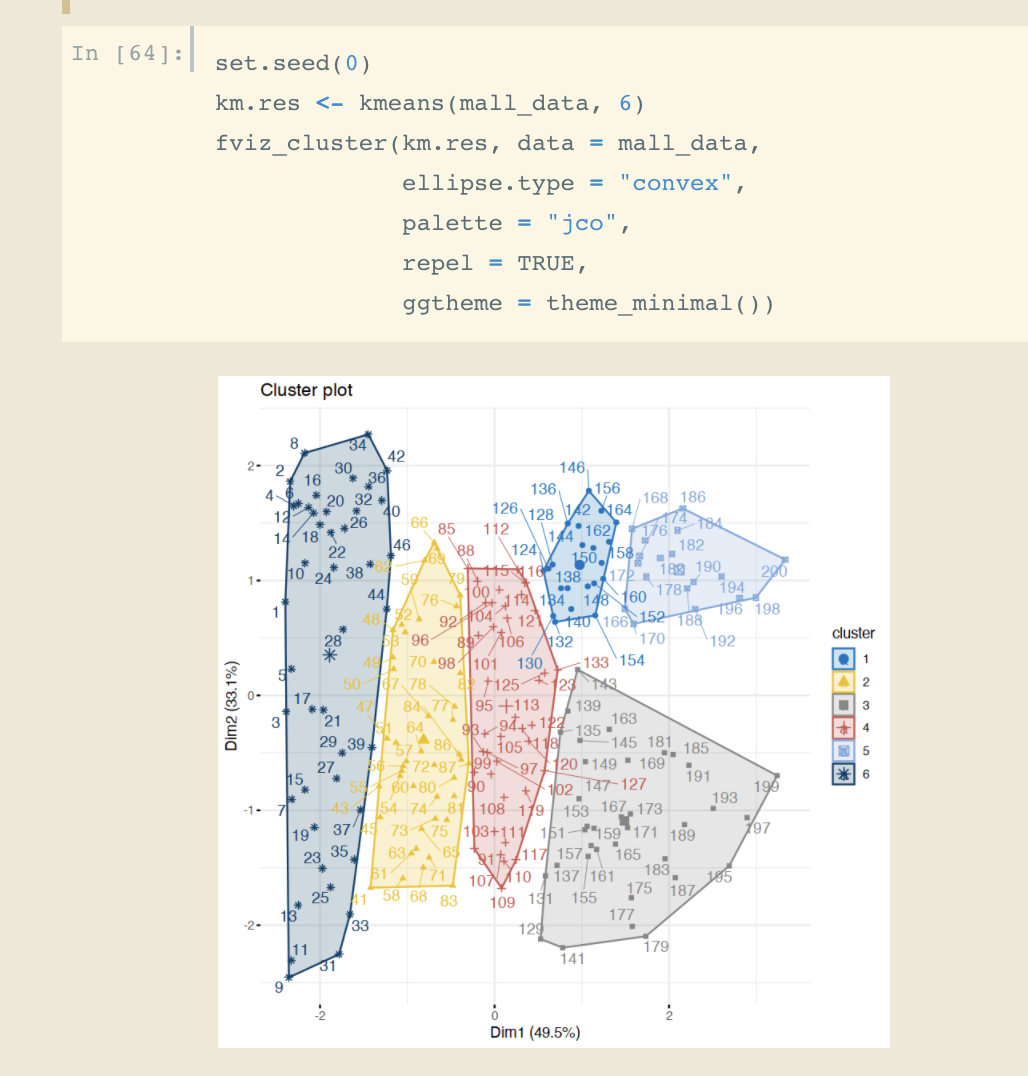
\includegraphics[width=0.65\textwidth]{k3}
                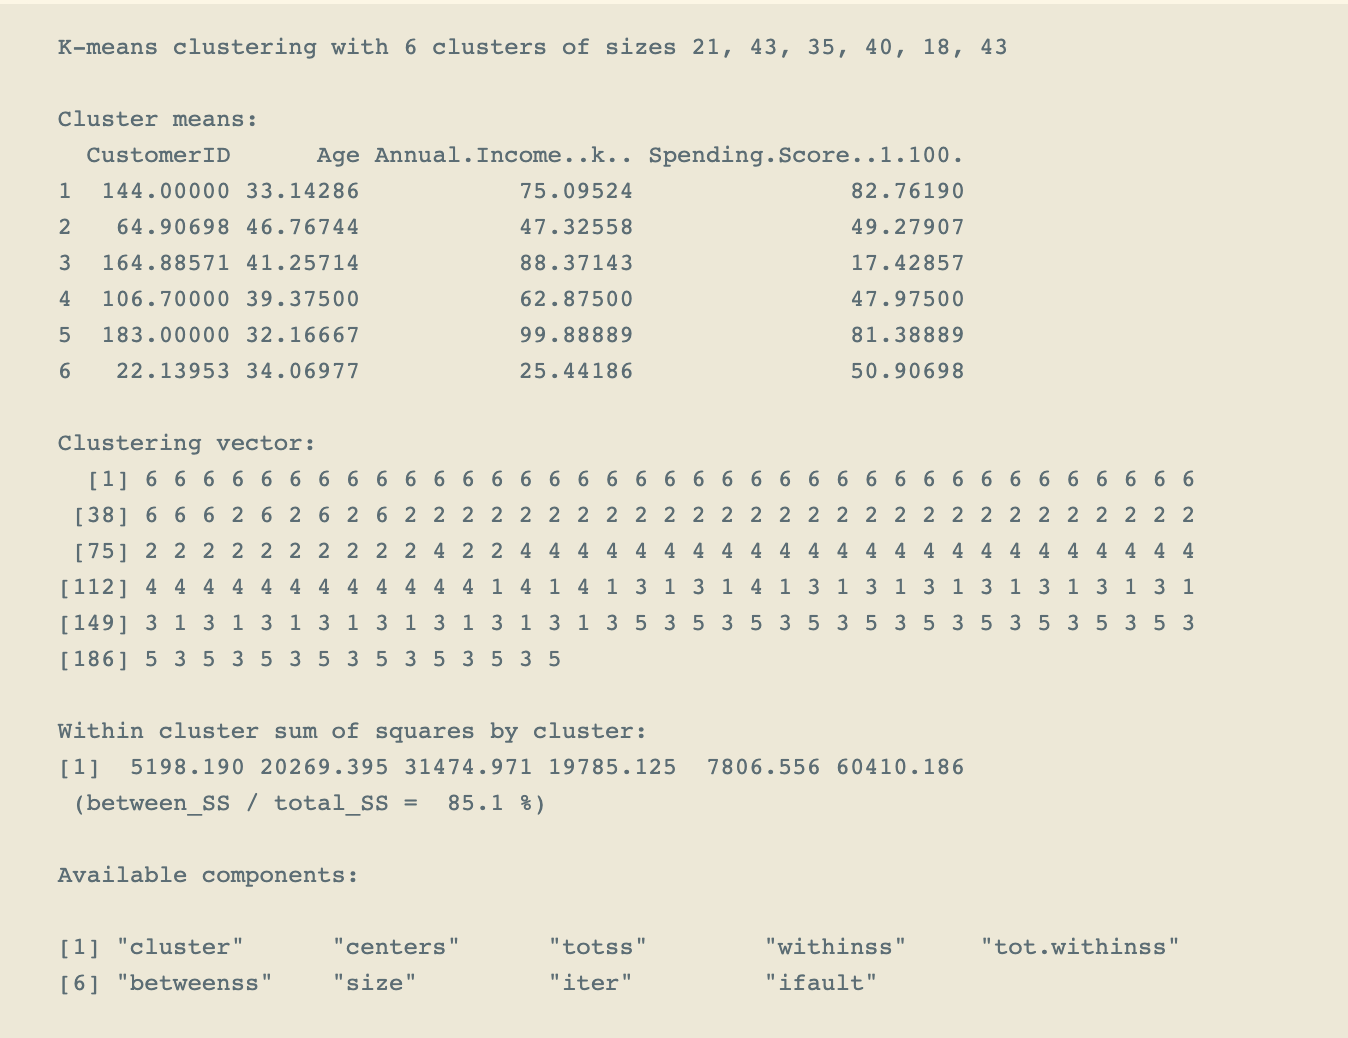
\includegraphics[width=0.65\textwidth]{k31}
            \end{figure}

            El algoritmo K-Means generó los siguientes 6 grupos:
            \begin{itemize}
                \item clientes más jóvenes con puntaje de gasto  medio  anual y  medio 
                \item clientes con  alto  ingreso anual y  bajo  puntaje de gasto
                \item clientes más jóvenes con puntaje de gasto  medio  anual y  medio 
                \item clientes con  altos  ingresos anuales y  alto  puntaje de gastos
                \item clientes con  bajo  ingreso anual y  bajo  puntaje de gasto
                \item clientes con  bajo  ingreso anual y  alto puntaje de gasto
            \end{itemize}

            No hay grupos distintos en términos de edad de los clientes.

    \clearpage
    \section{Técnica: DBSCAN}
        \subsection{Historia y funcionamiento}

        El clustering basado en la densidad utiliza la idea de de densidad y conectividad de densidad
        (como alternativa a la medición de distancia), lo que la hace muy útil para descubrir un grupo en 
        formas no lineales. 
        
        Este método encuentra un área con una densidad más alta que el área restante. 
        Uno de los métodos más famosos es la Agrupación espacial basada en densidad de aplicaciones con ruido 
        (DBSCAN). Utiliza el concepto de accesibilidad de densidad y conectividad de densidad.

        El algoritmo de agrupamiento basado en densidad DBSCAN es una técnica fundamental de agrupamiento de datos para 
        encontrar grupos de formas arbitrarias, así como para detectar valores atípicos.

        A diferencia de K-Means, DBSCAN no requiere el número de clústeres como parámetro. Más bien, infiere el número 
        de grupos basados en los datos, y puede descubrir grupos de forma arbitraria (en comparación, K-Means 
        generalmente descubre grupos esféricos). Los métodos de partición (K-means, agrupación PAM) y la agrupación 
        jerárquica son adecuados para encontrar agrupaciones de forma esférica o agrupaciones convexas. En otras palabras,
        funcionan bien para grupos compactos y bien separados. Además, también se ven gravemente afectados por 
        la presencia de ruido y valores atípicos en los datos.

        \subsection{Ventajas y desventajas}

        Las ventajas de la agrupación basada en la densidad son:
        \begin{itemize}
            \item No se asume el número de grupos. El número de grupos a menudo se desconoce de antemano. 
            Además, en un flujo de datos en evolución, el número de grupos naturales a menudo está cambiando.
            \item Descubrimiento de racimos con forma arbitraria. Esto es muy importante para muchas aplicaciones de flujo de datos.
            \item Capacidad para manejar valores atípicos (resistente al ruido).
        \end{itemize}

        Las desventajas de la agrupación basada en la densidad son:
        \begin{itemize}
            \item Si hay variación en la densidad, no se detectan puntos de ruido
            \item Sensible a los parámetros, es decir, difícil de determinar el conjunto correcto de parámetros.
            \item La calidad de DBSCAN depende de la medida de distancia.
            \item DBSCAN no puede agrupar bien los conjuntos de datos con grandes diferencias de densidad.
        \end{itemize}
        
        Una limitación de DBSCAN es que es sensible a la elección de e, en particular si los 
        grupos tienen densidades diferentes. Si e es demasiado pequeño, los grupos más dispersos 
        se definirán como ruido. Si e es demasiado grande, los grupos más densos pueden fusionarse.

        \clearpage
        \subsection{Apliquemoslo a los datos}   

            \subsubsection{¿Qué parametros usar?}

            Para encontrar el parametro de dbscan usaremos una funcion ya establecida:
            \begin{figure}[ht!]
                \centering
                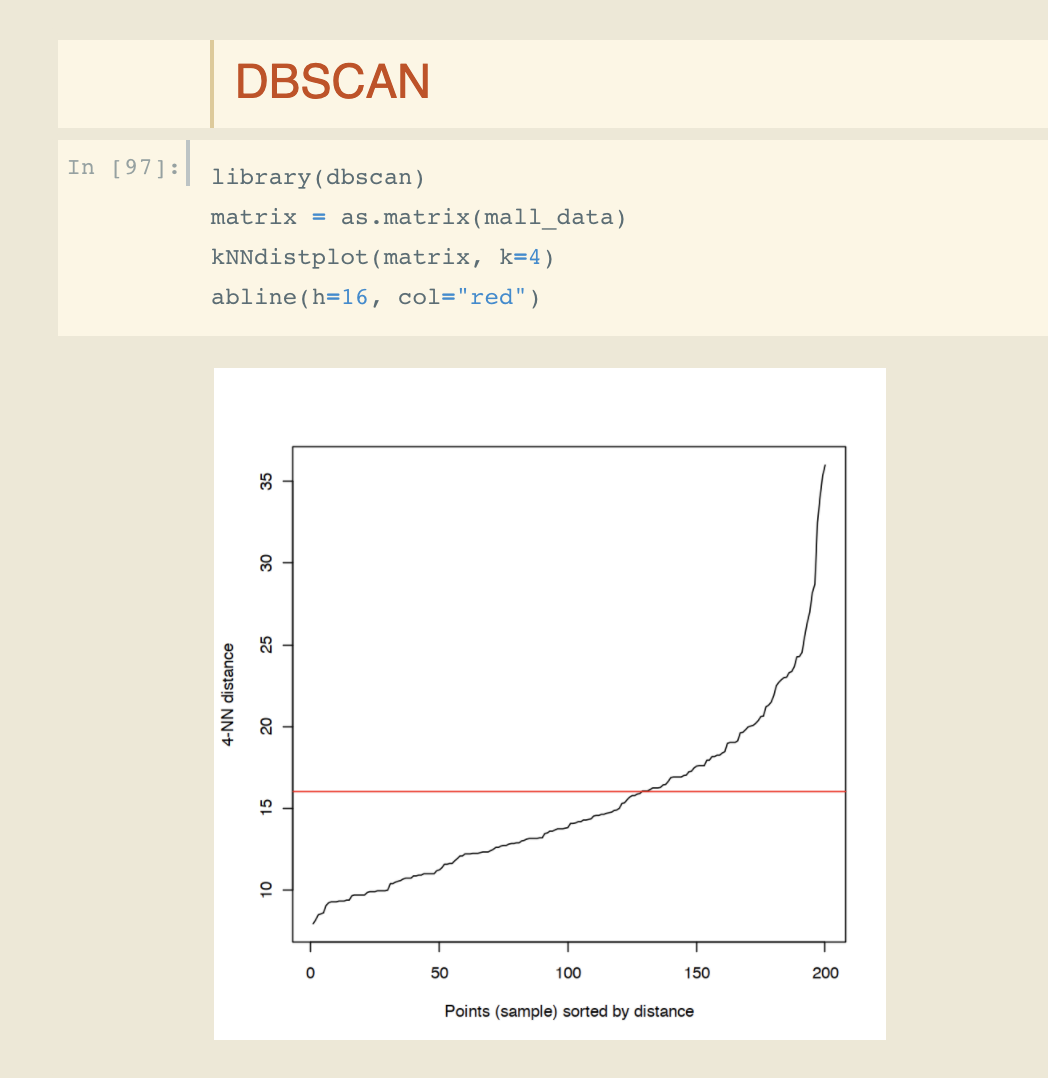
\includegraphics[width=0.75\textwidth]{d1}
            \end{figure}

            Esta de una resultado entre el que e = $13 +- 3$, veamos los resultados de usarlo:
            \begin{figure}[ht!]
                \centering
                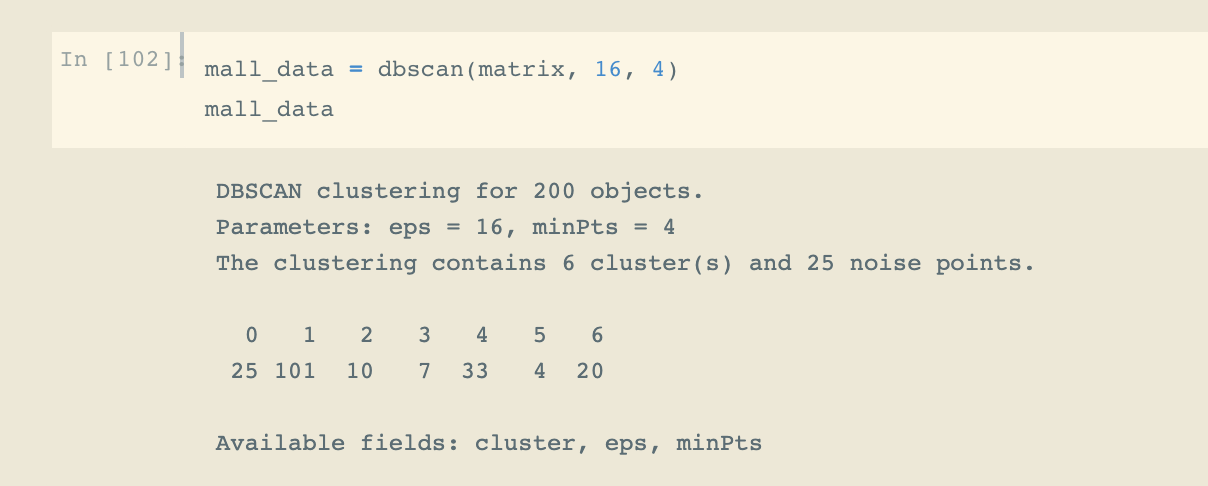
\includegraphics[width=0.85\textwidth]{d2}
                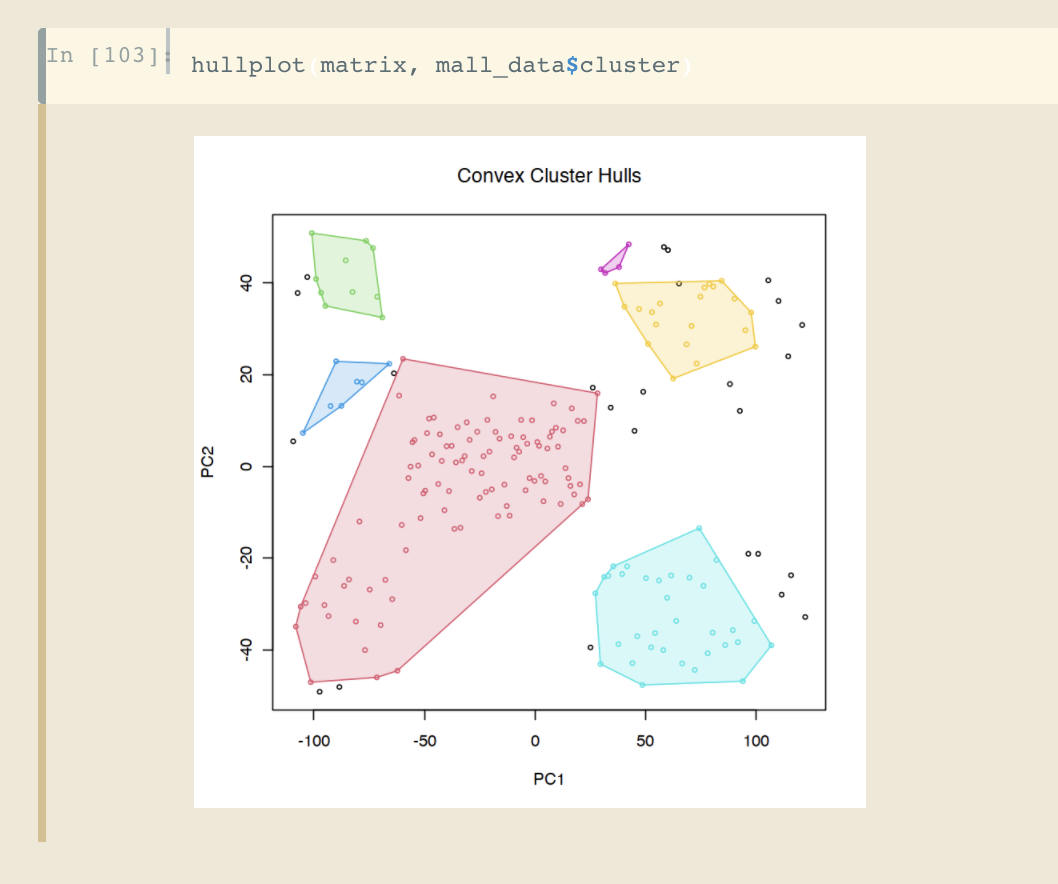
\includegraphics[width=0.85\textwidth]{d3.png}
            \end{figure}

            DBSCAN encontro entonces 6 clusters y uno de ruido, estos tienen una variacion muy grande, hay 25 puntos que clasifico como ruido.
            En la grafica podemos ver cuales fueron esos outliers, puntos que no tienen la distancia ni la cantidad de datos necesarios para 
            ser un cluster.

            Y aqui es donde la cosa se puso fea, porque no encontre algo que uniera a los clusters, por un lado por falta de tiempo pero
            tambien porque no encuentro una característica comun para los clusters que DBSCAN hizo.


    \section{Posibles mejoras a futuro}

        \begin{itemize}
            \item Me puse a investigar mucho sobre un algoritmo conocido como "Affinity Propagation" y siento que seria una gran comparación usarlo.
            \item Encontrar un patrón sobre los clusters de DBSCAN.
        \end{itemize}

    \section{Conclusión}

    Gracias a los resultados vimos está claro que DBSCAN no pudo generar grupos razonables.
    Se debe a sus problemas para reconocer grupos de varias densidades (que están presentes en este caso).
    
    A su vez, el algoritmo de K-Means creo 5-6 grupos razonables y que se pudieron con algo de análisis encontrar a que
    grupos correspondían.
    
    \section{Evidencia}
    
    Por si quieres corroborar todo lo que aquí se experimento deje adjunto una libreta que puedes usar para jugar con le código
    

\begin{thebibliography}{10}

  \bibitem{1} 
      \textit{k MEANS}, 
      \url{https://www.datanovia.com/en/courses/advanced-clustering/}

  \bibitem{2} 
      \textit{DBSCAN}, 
      \url{https://www.datanovia.com/en/lessons/dbscan-density-based-clustering-essentials/}

\bibitem{3}
    \textit{Anthony Botibol}, 
    The Importance of Customer Segmentation\\
    https://www.bluevenn.com/blog/the-importance-of-customer-segmentation

\end{thebibliography}



\end{document}